\documentclass[12pt,a4paper]{report}


\usepackage[italian]{babel}
\usepackage{todonotes}

% Set page size and margins
% Replace `letterpaper' with `a4paper' for UK/EU standard size
\usepackage[letterpaper,top=2cm,bottom=2cm,left=3cm,right=3cm,marginparwidth=1.75cm]{geometry}

% Useful packages
\usepackage{amsmath}
\usepackage{float}
\usepackage{graphicx}\usepackage{array}
\newenvironment{conditions}
  {\par\vspace{\abovedisplayskip}\noindent\begin{tabular}{>{$}l<{$} @{${}={}$} l}}
  {\end{tabular}\par\vspace{\belowdisplayskip}}
\usepackage[colorlinks=true, allcolors=black]{hyperref}
\usepackage[T1]{fontenc}
\usepackage[utf8]{inputenc}
\usepackage{setspace}
\usepackage[paper=a4paper,margin=1in]{geometry}
\usepackage[square,numbers,super]{natbib}
\usepackage[nottoc]{tocbibind}
\makeatletter
\renewenvironment{abstract}{%
    \if@twocolumn
      \section*{\abstractname}%
    \else
      \begin{center}%
        {\bfseries \Large\abstractname\vspace{\z@}}
      \end{center}%
      \quotation
    \fi}
    {\if@twocolumn\else\endquotation\fi}
\makeatother

\begin{document}


\begin{titlepage}
        
        \noindent
        \begin{minipage}[t]{0.19\textwidth}
            \vspace{-4mm}{
\includegraphics[scale=1.15]{logo_unimib.pdf}}
        \end{minipage}
        \begin{minipage}[t]{0.81\textwidth}
        {
                \setstretch{1.42}
                {\textsc{Università degli Studi di Milano - Bicocca}} \\
                \textbf{Scuola di Scienze} \\
                \textbf{Dipartimento di Informatica, Sistemistica e Comunicazione} \\
                \textbf{Corso di laurea in Informatica} \\
                \par
        }
        \end{minipage}
        
	\vspace{40mm}
        
	\begin{center}
            {\LARGE{
                    \setstretch{1.2}
                    \textbf{Strategie di automatizzazione di liquidità nella finanza decentralizzata}
                    \par
            }}
        \end{center}
        
        \vspace{40mm}

        \noindent
        {\large \textbf{Relatore:} Prof. Alberto Leporati } \\
        
         \noindent
        {\large \textbf{Correlatore:} Ing. Paolo Antonio Rossi}
        
        \vspace{15mm}

        \begin{flushright}
            {\large \textbf{Relazione della prova finale di:}} \\
            \large{Christian Kobril} \\
            \large{Matricola 856448} 
        \end{flushright}
        
        \vspace{40mm}
        \begin{center}
            {\large{\bf Anno Accademico 2021-2022}}
        \end{center}

        \restoregeometry
        
    \end{titlepage}


\begin{abstract}
   Qui scrivo il sommario
\end{abstract}
\tableofcontents






\chapter{Introduzione}
\todo{prima frase forse non adatta}
\noindent Il tema centrale di questa Tesi di Laurea è la \textbf{finanza decentralizzata}.\\ In particolare, si approfondirà il ruolo che la blockchain ha in questo settore, presentando un prodotto software concretamente sviluppato durante il mio  \textit{Project Work}, svolto presso l'azienda \textit{Five Elements Labs Srl}.
\\\\Inoltre, verranno approfonditi i concetti di \textit{pool di liquidità}, \textit{automated market maker(AMM)} e \textit{strategie multiple} su Uniswap V3.

\todo{pensare ad un titolo più adeguato per la sezione}
\section{Un breve sguardo alla tecnologia}

Alla base di tutti i protocolli e prodotti software analizzati in questa Tesi, vi è un minimo comune denominatore che prende il nome di \textbf{blockchain}\cite{blockchain}.
\\La blockchain altro non è che un database (o in termini contabili, \textit{libro mastro}) \textbf{condiviso} tra più nodi di una rete, \textbf{validati} dalla rete stessa e strutturato come una catena di blocchi contenenti delle \textbf{transazioni}.
\\\\Sostanzialmente possiamo riassumere le funzionalità di questa rete di blocchi in 3 importanti concetti:

\begin{itemize}
  \item \textbf{tracciabilità} - tutti i partecipanti alla rete e le transazioni registrate devono poter essere rintracciabili
  \item \textbf{immutabilità} - una volta che una transazione viene salvata sulla blockchain, non può essere in alcun modo alterata
  \item \textbf{sicurezza} - la crittografia asimmetrica utilizzata nella rete garantisce invio e ricezione di transazioni in modo sicuro, senza bisogno di intermediari esterni
\end{itemize}

\noindent Questa recente tecnologia è oggi in \textbf{piena crescita}: vi sono numerose aziende e sviluppatori indipendenti che costruiscono prodotti innovativi e ad altissimo potenziale, basati sulla blockchain.


\subsection{Le dimensioni del mercato attuale}
\todo{sezione troppo orientata ad economia?}

\noindent Nel 2021, secondo un report di \textbf{Electric Capital}\cite{web3_dev} mostrato nell'immagine \ref{fig:web3_dev} è stata raggiunto un nuovo record di \textbf{18.000 sviluppatori attivi al mese} nello sviluppo di software basati su blockchain. \\Si stima inoltre che più del \textbf{65\%} degli sviluppatori blockchain abbia iniziato a lavorare nel 2021 in questo nuovo settore, con un aumento di \textbf{34.000} persone, il più alto nella storia.

\begin{figure}[H]
  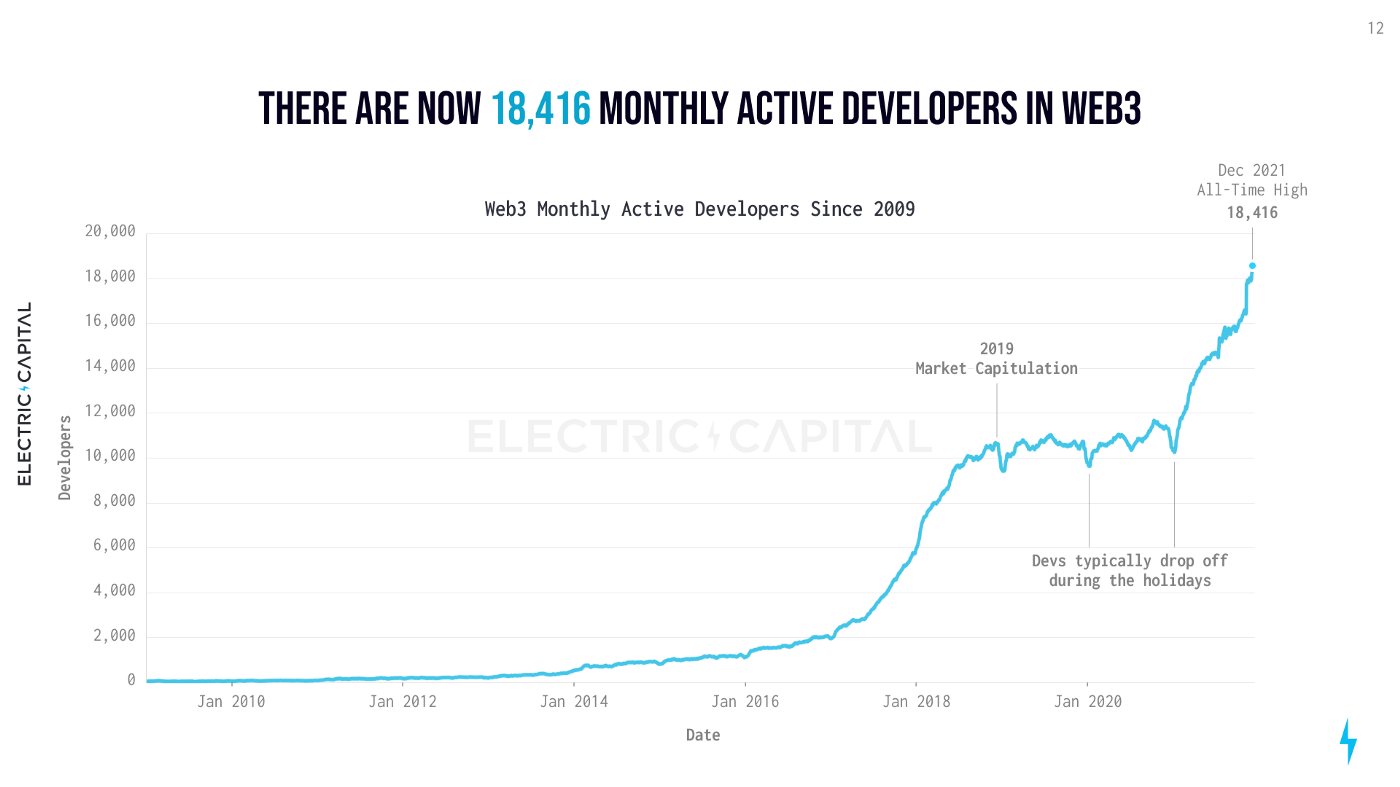
\includegraphics[scale=0.3]{web3_dev.png}
  \centering
  \caption{Crescita del numero di sviluppatori nel settore Web3 secondo Electric Capital}
  \label{fig:web3_dev}
\end{figure}

\todo{personalmente credo da cambiare con qualcos'altro}
\noindent Personalmente credo che questo forte aumento di sviluppatori sia dovuto allo \textbf{scoppio} della tecnologia \textbf{NFT} e al rapido crescere del valore delle principali cripto valute, \textbf{Bitcoin} e \textbf{Eth}, che nel 2021 hanno raggiunto il massimo storico, attirando l'attenzione sul mercato e mettendo in luce il potenziale di questa innovativa tecnologia.

\section{Cos'è la Finanza Decentralizzata}

Il termine \textbf{finanza decentralizzata} viene usato per classificare tutti quei servizi finanziari che avvengono direttamente tra due entità su una blockchain.

\subsection{Differenze tra Finanza Decentralizzata e Tradizionale}

Per comprendere il concetto su cui si basa la finanza decentralizzata (da ora in poi \textit{DeFi}), è bene dare un rapido sguardo alla sua controparte: la finanza tradizionale (o centralizzata).\\\\
Nella finanza centralizzata, ogni singola operazione finanziaria tra due persone (bonifici, prestiti, scambio di risorse, mutui) richiede l'interazione con soggetti di terze parti (tipicamente banche o altri enti).\\
Ciò incrementa le già prolisse tempistiche burocratiche, oltre ad aggiungere i costi dovuti al servizio fornito dagli enti che permettono l'operazione.
\\\\Invece, la finanza decentralizzata permette l'interazione tra due soggetti senza l'intermediazione di un sistema centralizzato, bensì mediante un applicativo software costruito sopra la tecnologia blockchain, rendendo le operazioni rapide, pubbliche e sicure.


\section{Caratteristiche e vantaggi della DeFi}

\subsection{Applicazioni decentralizzate}
Gli applicativi software utilizzati in DeFi vengono chiamati \textit{dApps (decentralized applications)}, ovvero particolari prodotti che interagiscono con diverse blockchain. Di tali reti noi considereremo solo quella di \textbf{Ethereum}\cite{ethereum}, nota per la sua flessibilità e accessibilità.\\\\
\todo{dare più contesto su ethereum}
La blockchain di Ethereum, a differenza di reti come quella di \textbf{Bitcoin}\cite{bitcoin}, è \textbf{programmabile}; ossia è possibile costruirci sopra e distribuire dApps, rendendo la rete una sorta di gigantesco marketplace in cui trovare servizi finanziari, videogiochi, social network e diverse altre applicazioni.
\todo{cosa fanno gli smart contract, approfondisco}
\\Su tale blockchain risiedono dei particolari programmi denominati \textit{Smart Contracts}\cite{smartcontracts}, i quali sono costruiti come un insieme di dati e funzioni, che risiedono ad uno specifico indirizzo sulla rete Ethereum.

\todo{Spiego EVM}

\subsection{Accesso alle dApps}

Il concetto di login ideato nel web tradizionale (noto anche come Web2), tipicamente caratterizzato dall'inserimento di un'email e una password, viene sorpassato da una nuova autenticazione del \textbf{Web3}\cite{web2_web3}: attraverso il proprio \textit{portafoglio digitale} (da ora in poi, wallet \cite{wallet}) è possibile accedere al proprio account e gestire i propri assets digitali, eventualmente mettendoli a disposizione della dApp a cui si è connessi.
\\\\I wallet presentano il vantaggio di non dover fornire nomi, indirizzi fisici, email o altre informazioni personali, garantendo la riservatezza dei propri dati; basta creare un wallet per avere immediato accesso alle piattaforme, senza registrazioni.



\subsection{Operazioni in DeFi}
\todo{non sono operazioni SOLO in DeFi, si può spiegare meglio}
Ogni operazione nella DeFi viene detta \textbf{transazione}. Una transazione è permanentemente salvata sui registri della blockchain, rendendo ogni singola operazione, associata ad un identificativo, consultabile in qualsiasi momento da qualsiasi persona.
\\Tale trasparenza viene difficilmente concessa dalle banche, ponendo la DeFi come un sistema aperto e rintracciabile.

\subsection{Flessibilità}

L'ultima caratteristica della DeFi che ritengo importante citare è ciò che più la contraddistingue dalla finanza tradizionale: la sua flessibilità.\\
In qualsiasi momento un utente può trasferire i propri assets digitali, senza dover chiedere il permesso a soggetti di terze parti, evitando costose commissioni e con un'attesa che va da pochi secondi a pochi minuti. 


\chapter{Uniswap, piattaforma di Liquidity Providing}

\todo{intro da rivedere}
Avendo approfondito cosa è la DeFi, quali sono le sue caratteristiche e i principali vantaggi, ritengo necessario concentrarsi su quali sono i prodotti "dApps" che hanno messo le basi per il lavoro svolto durante il mio Project Work.

\section{Uniswap}

\todo{intro su uniswap da rivedere}
Innanzitutto, è bene distinguere la piattaforma Uniswap\cite{uniswap} dall'omonimo protocollo.
\\La dApp di Uniswap (conosciuta come Uniswap Interface) è una piattaforma che permette agli utenti l'interazione con il protocollo Uniswap.
\\\\Quest'ultimo è una suite di Smart Contracts, per definizione persistenti e non aggiornabili, che insieme formano un \textbf{Automated Market Maker} (da ora in poi AMM)\cite{amm}.

\section{Scambi nei mercati tradizionali}

La maggior parte dei mercati tradizionali ad accesso pubblico utilizza ciò che viene definito \textit{Order Book}\cite{order_book}, ossia un elenco degli ordini di acquisto e vendita attualmente aperti per un asset, organizzati per prezzo.
\todo{non spiego cosa sia un asset}
\\Sostanzialmente, un \textit{sistema di corrispondenza}\cite{matching} si occupa di abbinare gli ordini di acquisto con quelli di vendita, usando l'order book per eseguire le operazioni tra i partecipanti dello scambio.


\section{Automated Market Maker}

La rivoluzione introdotta dalla blockchain sta nella possibilità di creare nuovi tipi di scambi che abbinano algoritmicamente ordini di acquisto e vendita utilizzando gli smart contracts.
\\Tali scambi vengono detti \textit{Scambi Decentralizzati (DEX)}.
\\\\Un AMM è un protocollo DEX che si basa su un algoritmo di valutazione per prezzare gli asset mediante una formula matematica.
\\Il citato order book viene rimpiazzato con una pool di liquidità\cite{liquidity_pool}, contenente due asset, entrambi valutati l'uno rispetto all'altro.
\\Quando un asset viene scambiato per un altro, i prezzi relativi dei due asset cambiano, e viene determinato un nuovo tasso di mercato per entrambi.
In questo modo acquirenti e venditori interagiscono direttamente con la pool (e di conseguenza gli smart contracts), senza dover interagire tra di loro in modo diretto.

\subsection{Esempio pratico di AMM}

Un esempio pratico che mi ha aiutato a comprendere il funzionamento degli AMM è quello dei contadini di mele e patate.
\\Immaginiamo di essere un contadino e di avere solo patate, senza la possibilità di coltivare, e di conseguenza mangiare, nient'altro.\\ Un giorno ci viene proposto di effettuare degli scambi con un venditore di mele attraverso un messaggero, il quale decide di custodire mele e patate in un \textit{contenitore magico}, in modo tale che rimangano a disposizione per gli scambi.
\\\\La regola fondamentale per questo scambio è una sola: \textit{il contenitore magico dovrà sempre contenere lo stesso valore di mele e patate.}
\\Tale regola è in realtà la formula alla base dell'AMM di Uniswap, conosciuta come \textbf{Constant Product Formula} \ref{eqn:const_prod_f} (rappresentata graficamente nella figura \ref{fig:const_prod}): \\

\begin{equation}
x * y = k
\label{eqn:const_prod_f}
\end{equation}
dove:
\begin{conditions}
 x & numero di mele nel contenitore \\
 y & numero di patate nel contenitore \\  
 k & valore costante \\
\end{conditions}

\noindent \\In genere la costante $k$ è detta \textbf{liquidità} del contenitore.

\begin{figure}[H]
  \includegraphics[scale=0.40]{const_prod.png}
  \centering
  \caption{Grafico della Constant Product Formula applicata all'esempio dei contadini}
  \label{fig:const_prod}
\end{figure}

\noindent\\Inizialmente il contenitore sarà perfettamente bilanciato, per esempio con 500 mele e 500 patate corrispondente ad una liquidità ($k$) pari a 250.000.

\subsection{Scambi nel contenitore}

\\\\Immaginiamo ora che un contadino voglia scambiare le sue patate per delle mele grazie al contenitore.
Poniamo che il numero di patate offerte dal contadino sia pari a \textit{70}.
Ricordando che la costante $k$ deve sempre corrispondere a \textit{250.000}, il calcolo per la quantità di mele che dovrà essere presente nel contenitore è:\\


\begin{equation}
M_{n} = \frac{k}{P_{0}_ + P_{1}}
\label{eqn:nuove_mele}
\end{equation}
dove:
\begin{conditions}
 M_{n} & nuova quantità di mele nel contenitore \\
 P_{0} & quantità iniziale di patate nel contenitore \\  
 P_{1} & quantità di patate inviate
\end{conditions}

\noindent \\\\Questo perché per bilanciare il contenitore mantenendo il valore k costante, il numero di mele deve diminuire, e di conseguenza il prezzo delle mele stesse aumentare.
Dunque, il nuovo numero di patate nel contenitore corrisponde a \textit{570}, mentre il numero di mele, calcolato mediante la \textbf{formula \ref{eqn:nuove_mele}} è uguale a \textit{438}: di conseguenza il contadino riceverà \textit{500 - 438 = 62 mele}.
\\Allo stesso modo, se un contadino volesse scambiare le proprie mele, riceverebbe più patate rispetto alle mele inviate, considerato l'aumento del prezzo della mela rispetto alle patate.
\\\\Nella realtà dei fatti, questo contenitore magico è conosciuto come \textbf{pool di liquidità}.

\section{Pool di liquidità}

È possibile vedere una pool di liquidità come uno spazio in cui i contandini (trader) possono mettere a disposizione la propria liquidità di mele e patate (criptovalute, nello specifico token ERC-20\cite{erc_20}); tali utenti vengono definiti fornitori di liquidità (\textit{liquidity providers, da ora in poi LP}).
\\\\Come ricompensa per la liquidità fornita, gli \textbf{LP} ricevono commissioni sulle operazioni che avvengono nella pool a cui partecipano. 
Tali commissioni si applicano sulle singole transazioni effettuate con la liquidità fornita da un LP, e possono variare di percentuale dal 0.01\%\ fino all'1\%\.\\\\Nel caso di Uniswap, gli LP depositano un valore equivalente di due token; per esempio, 50\% ETH e 50\% USDC (una stablecoin che replica il dollaro USA) nella pool ETH/USDC.


\section{Protocollo Uniswap V3}

Uniswap V3 è l'ultima versione del protocollo rilasciata da Uniswap nel maggio 2021.\\ Tale protocollo definisce le funzionalità della suite di smart contracts con cui gli utenti interagiscono, introducendo importanti novità rispetto al suo predecessore, V2.

\subsection{Posizioni}

Utilizzando l'interfaccia Uniswap, gli utenti possono connettere il loro wallet personale per mettere a disposizione un certo ammontare di liquidità all'interno di una pool.
\todo{equa proporzione, come mai?}
Tale liquidità, come spiegato in precedenza, dovrà mantenere un'equa proporzione tra i due asset messi a disposizione: tale operazione viene definita come \textit{apertura di una \textbf{posizione}} (o in inglese, position minting).
\\\\Su Uniswap V3, le posizioni vengono rappresentate mediante NFT (ERC-721\cite{erc_721}), i quali certificano un determinato wallet, in questo caso chi effettua il minting, come proprietario della posizione.

\subsection{Complicazioni di Uniswap V2}

\\\\In precedenza, nella V2 di Uniswap, i LP mettevano a disposizione i propri asset per scambi \textbf{a qualsiasi intervallo di prezzo}.
\\\\Consideriamo che io, trader che utilizza Uniswap V2, voglia mettere a disposizione due miei asset chiamati token $A$ e token $B$.
Ricordando che l'intervallo di prezzo è sempre il prezzo di $A$ rispetto al prezzo di $B$ ($A$ \textbf{su} $B$), in questa versione del protocollo la liquidità viene uniformemente distribuita su tutti i prezzi possibili.
\\In questo modo non vi è alcuna perdita di liquidità, portando però un importante svantaggio: la maggior parte della liquidità non viene mai utilizzata negli scambi.
\\\\Provando a considerare una pool contenente una coppia di due stable coins, ossia token il cui prezzo rimane relativamente costante nel tempo (ad esempio, USDC vale quanto il dollaro americano), possiamo essere certi che la liquidità al di fuori del tipico intervallo di prezzo dei suddetti stable coins non verrebbe mai utilizzata.
\\\\Per esempio in Uniswap V2 la coppia DAI/USDC (\textbf{entrambi stable coins dal valore di circa \$\01}) utilizza circa il 0.50\%\ del capitale totale disponibile per gli scambi all'interno del range tra \$\00.99 e \$\11.01\cite{v2_waste}. Il resto della liquidità è distribuito nella restante fascia di prezzo tra 0 e $\infty$ (escluso il range sopra citato), rendendo quel capitale inutilizzabile (e dunque, non consentendo agli LP di guadagnare commissioni). 
\\\\Ciò è dovuto al fatto che la liquidità sia uniformemente distribuita in un range di prezzo da 0 a $\infty$, e non \textit{concentrata} nel giusto intervallo: per tale ragione è stato introdotto \textbf{Uniswap V3}.

\subsection{Liquidità concentrata}
\\\\Ciò che rende Uniswap V3 un protocollo davvero valido è l'idea della \textit{Liquidità Concentrata}\cite{concentrated_liquidity}. Tale liquidità viene distribuita in un intervallo di prezzo personalizzabile, a scelta dell'utente.
\\\\Riprendendo l'esempio sopra citato, un trader potrebbe decidere di investire nella pool DAI/USDC, scegliendo come range il più proficuo, ossia quello compreso tra \$\00.99 e \$\11.01.
In tal modo, la liquidità concentrata garantirà un guadagno superiori di commissioni (da ora in poi fees) sfruttando il capitale messo a disposizione dai LPs.

\subsection{Tick di prezzo}

Per rendere la liquidità concentrata funzionale, lo spazio continuo del prezzo è stato partizionato in \textbf{tick}.
\\\\I tick sono i limiti di aree discrete nello spazio del prezzo. Tali limiti sono posizionati in modo tale che il diminuire o aumentare di 1 tick rappresenti l'aumento o la diminuzione percentuale del 0.01\%\ del prezzo in ogni punto dello spazio.
\\Dunque quando una posizione viene creata, un LP non può scegliere qualsiasi valore per il range di prezzo: è necessario che il limite inferiore (\textbf{lower tick}) e il limite superiore (\textbf{upper tick}) corrispondano a dei tick di prezzo validi.

\subsection{Swap e Fees}

Il modo più utilizzato per interagire con Uniswap V3 è tramite gli scambi (da ora in poi \textbf{swap}).
Uno swap è relativamente semplice: un utente seleziona un token ERC-20 del quale è proprietario e un token che vorrebbe scambiare per esso. Uniswap venderà il token attualmente in possesso dell'utente, restituendo una quantità proporzionale del token desiderato, sottraendo una \textbf{swap fee}, ossia quella percentuale riconosciuta ai LPs per aver messo a disposizione la loro liquidità con la quale è avvenuto lo scambio.
\\\\Tuttavia, la transazione potrebbe richiedere alcuni minuti, a seconda della rete su cui avviene, rilevando un fenomeno conosciuto come \textbf{slippage}.
\\Lo slippage è l'alterazione di prezzo di un token che avviene mentre la transazione è in attesa di essere completata. Tale alterazione ha una soglia di tolleranza dell'1\%\: superata tale soglia l'operazione viene rifiutata e lo swap annullato, onde evitare grosse perdite per l'utente.

\section{Complicazioni di Uniswap V3}

Qualora il prezzo di un token dovesse muoversi verso una direzione (di discesa o di salita), il proprietario della posizione si ritroverebbe con un ammontare superiore di uno dei due token rispetto all'altro, in quanto il prezzo dell'uno sull'altro cambierà, fino a quando l'intera liquidità sarà relativa a solo uno dei due asset.
\\\\Per esempio, se in una pool ETH/USDC il prezzo di ETH dovesse diminuire, la percentuale di liquidità relativa a ETH aumenterebbe, per bilanciare il valore immesso all'interno della posizione stessa.
Allo stesso modo, se ETH dovesse aumentare di valore, la percentuale di USDC aumenterebbe a sua volta.
\\\\Con l'aumentare o il diminuire del prezzo di un asset nella pool, tale prezzo potrebbe uscire dall'intervallo che un LP ha impostato per una certa posizione. Nel momento in cui una posizione si dovesse trovare fuori dall'intervallo scelto (\textbf{Out Of Range position}) la liquidità diventerebbe inattiva (\textbf{idle liquidity}) e l'utente proprietario di tale liquidità non guadagnerebbe più fees.
\\Tuttavia, nel momento in cui il valore del primo token sul secondo dovesse tornare nell'intervallo di prezzo iniziale, il LP tornerebbe a guadagnare fee.
\\\\È proprio dal problema della liquidità inattiva che nasce \textbf{Orbit DeFi}, il prodotto sviluppato durante il mio project work.







\chapter{Orbit, piattaforma per automatizzare strategie DeFi}

Ho avuto l'opportunità di svolgere il mio Project Work per Five Elements Labs, azienda specializzata nella produzione di software nel mondo blockchain; in particolare nei settori DeFi e NFT.
\\Durante tale esperienza, mi sono unito allo sviluppo del loro principale prodotto: \textbf{Orbit}\cite{orbit_website}.

\section{Introduzione ad Orbit}


\textbf{Orbit} è una piattaforma di gestione di liquidità nel settore DeFi: ossia un \textbf{layer} che permetta ai propri utenti di automatizzare strategie e di ottimizzare posizioni di liquidità su Uniswap V3.
\\Può essere interpretato come \textbf{un'estensione} del proprio wallet, in grado di gestire gli assets degli utenti per fornire la possibilità di ottenere un ritorno aggiuntivo dalla liquidità concentrata.

\section{Perché nasce Orbit}

Con il rapido crescere del settore DeFi e del corrispondente ecosistema di protocolli, ognuno con le proprie caratteristiche e logiche, risulta sempre più complesso gestire delle strategie di liquidità al passo con i tempi.

\subsection{Gas fee}
\\Ogni transazione avvenuta sulla blockchain ha un \textit{"costo"} chiamato \textbf{gas fee}\cite{gas}.
\\È possibile affermare che il gas sta alla blockchain come la \textbf{benzina} sta alla macchina; è necessario per far funzionare i nodi che compongono la rete.
\\Sostanzialmente è l'unità di misura dello \textit{sforzo computazionale} fatto dai nodi per sostenere una transazione, la quale può prevedere diverse complesse operazioni al suo interno.
\\Tale benzina deve essere in qualche modo pagata, per questo esistono commissioni sul gas (gas fee).
\\\\Diverse blockchain con basse gas fee (come \textbf{Polygon}\cite{polygon}) stanno diventando sempre più popolari, spostando l'attenzione degli sviluppatori e degli utenti verso la possibilità di costruire piattaforme e strumenti veloci ed efficaci.
\\\\Orbit dunque cavalca quest'onda di innovazione e di creatività, portando la liquidità concentrata verso un nuovo livello, costruendo uno strumento efficiente e facile da utilizzare per professionisti e novizi del mondo DeFi.\\\\

\section{Vantaggi per gli utenti}

Automatizzare strategie riguardo posizioni su Uniswap V3 ha un diretto impatto sui \textbf{ritorni generati} da queste ultime.
\\La maggior parte dei protocolli presenti sul mercato forniscono ai trader \textbf{strategie attive}, sulle quali è necessario compiere delle complesse scelte conosciute perlopiù da utenti professionisti.
\\\\Le funzionalità fornite da Orbit permettono agli utenti di creare \textbf{strategie passive}, senza il necessario bisogno di rimanere aggiornati sui protocolli, bensì lasciando alla piattaforma il compito di gestire la propria liquidità.
\\Inoltre, nella prima versione del protocollo, sarà Orbit ad occuparsi dei costi di gas dovuti alle transazioni rivolte agli smart contract dell'applicazione.

\section{Modelli di gestione di liquidità}

Nello stato attuale della DeFi, vi sono concretamente due modelli ben distinti di gestione di liquidità:  \textbf{Aggregatori}\cite{aggregator} e  \textbf{Smart Vaults}\cite{smart_vault}.

\subsection{Aggregatori}

Gli Aggregatori sono delle particolari piattaforme DeFi, le quali permettono ai propri utenti di effettuare transazioni verso diverse dApps \textbf{in un unico posto}. Ciò permette di risparmiare tempo e aumentare l'efficienza delle transazioni.
\\\\Tali Aggregatori permettono ai trader di \textbf{replicare} strategie di utenti esperti e di applicarle al proprio portfolio. Per esempio, possono confrontare i prezzi degli assets su diverse piattaforme, proponendo lo scambio più conveniente all'utente.
\\\\Tuttavia, protocolli utilizzatori di Aggregatori come \textit{Yearn Finance}, \textit{Beefy} o \textit{Idle} consentono all'utente l'utilizzo di strategie singole, tipicamente con un modello "\textit{Black Box}", ovvero senza verificarne l'effettivo funzionamento interno.

\subsection{Smarts vaults}

Contrariamente agli Aggregatori, gli \textbf{Smart Vaults} garantiscono un'alta \textbf{personalizzazione} delle strategie scelta direttamente dagli utenti.
\\Il funzionamento è relativamente semplice: un utente diventa \textit{proprietario} di un particolare Smart Contract effettuando una transazione che ne crea un'istanza contenente l'indirizzo del suo creatore.\footnote{Approfondimenti tecnici riguardanti la creazione dello Smart Vault e dei relativi Smart Contracts verranno trattati nel capitolo 5}.
\\Successivamente, il contratto creato viene utilizzato come \textit{un'estensione} del proprio wallet per gestire assets e per interagire con altri protocolli per consentire allocazioni automatiche di liquidità: tale Smart Contract è chiamato Smart Vault.
\\\\Il modello a Smart Vault è stato poco utilizzato in passato, principalmente a causa delle alte gas fee richieste dalle reti per attivare strategie multiple.
\\Tuttavia, con l'avvento di blockchain sempre meno costose in termini di gas, è ora possibile utilizzare gli Smart Vaults per integrare facilmente nuovi protocolli e fornire all'utente la possibilità di avere un totale controllo sulle interazioni con essi.
\\\\Per tali ragioni, il modello a Smart Vault è stato scelto per la realizzazione di Orbit.

\section{Moduli di Orbit}

La prima versione di Orbit rilasciata ad Agosto 2022 presenta 3 caratteristiche principali chiamate \textbf{moduli}: 

\begin{itemize}
  \item \textbf{Autocompound}
  \item \textbf{Autorebalance}
  \item \textbf{Idle liquidity}
\end{itemize}
\textbf{\list}
\noindent I moduli sono delle \textit{opzioni} attivabili su una determinata posizione di Uniswap V3 depositata nel proprio Smart Vault su Orbit. \\Ciascuno di tali moduli è rappresentato da uno smart contract, il quale innescherà delle specifiche \textbf{azioni} sulla base di determinati parametri relativi allo stato della posizione su cui agiscono.

\subsection{Autocompound module}

Il modulo di autocompound è sostanzialmente la traslazione verso il Web3 del \textit{compounding} nella finanza tradizionale. Il compounding si effettua quando un investitore decide di aggiungere gli interessi maturati da un investimento al capitale inizialmente investito, rendendoli a loro volta idonei per generare ulteriore interesse.
\\\\Nel mondo DeFi gli interessi generati sono le fee generate da una posizione, mentre il capitale investito è la liquidità messa a disposizione in una determinata pool.
\\Ricordiamo che i LP guadagnano fee su Uniswap V3 mentre i token delle posizioni da loro aperte si trovano in un determinato range di prezzo.
Il moduli di autocompound reinveste periodicamente le fee generate; tale operazione viene effettuata da bot esterni chiamati \textbf{keepers}.
\\Gli utenti più esperti possono scegliere delle soglie, superati le quali debba essere azionato il modulo di Autocompound, provocando il reinvestimento delle fee.
Per esempio, un utente può scegliere di innescare il modulo solo quando il valore delle fee generate supera il \textbf{5\%} del totale della liquidità investita nella posizione.
\\Nella tabella sottostante si può notare di quanto possa aumentare il \textbf{ritorno generato} con il modulo di Autocompound attivo (i dati sono presi da uno studio effettuato da Five Elements Labs): 
\\\\

\begin{center}
\begin{tabular}{ |p{5cm}|p{5cm}|p{2cm}| }
 \hline
 \multicolumn{3}{|c|}{Ritorno in percentuale} \\
 \hline
 Autocompund attivato& Autocompound disattivato &Differenza\\
 \hline
 5,00\%   & 4,89\%    &0,11\%  \\
 \hline
 10,00\%   & 9,57\%    &0,43\%  \\
 \hline
 15,00\%   & 14,06\%    &0,94\%  \\
 \hline
 20,00\%   & 18,37\%    &1,63\%  \\
 \hline
 30,00\%   & 26,50\%    &3,50\%  \\
 \hline
 40,00\%   & 34,10\%    &5,90\%  \\
 \hline
 60,00\%   & 47,93\%    &12,07\%  \\
 \hline
\end{tabular}
\end{center}
\\\\

\noindent \\Il modulo di autocompound presenta dunque un vantaggio per l'utente \textbf{incrementale}: più la posizione genera fee, più l'uso del modulo diventerà redditizio.
\subsection{Autorebalance module}

I successivi due moduli vertono su una delle maggior complicazioni di Uniswap V3: la \textbf{liquidità inattiva}.
\\Nel momento in cui questa Tesi sta venendo scritta, il \textbf{TVL} (\textit{Total Value Locked}, ossia capitale in DeFi) è pari a circa \textbf{\$10 miliardi}, rendendo la liquidità inattiva un problema non indifferente.\\
\\Il modulo di \textbf{autorebalance} permette di spostare il range di prezzo di una posizione che si trova fuori dal range di guadagno effettivo, centrandolo sul prezzo attuale del rapporto della coppia dei due Token presenti nella pool.
\\Nella figura \ref{fig:in_range}, si può notare come il prezzo attuale, rappresentato dallo spillo viola, si trovi attualmente all'interno del range verde. In questo caso, il proprietario della posizione sta guadagnando delle fee.


\begin{figure}[H]
  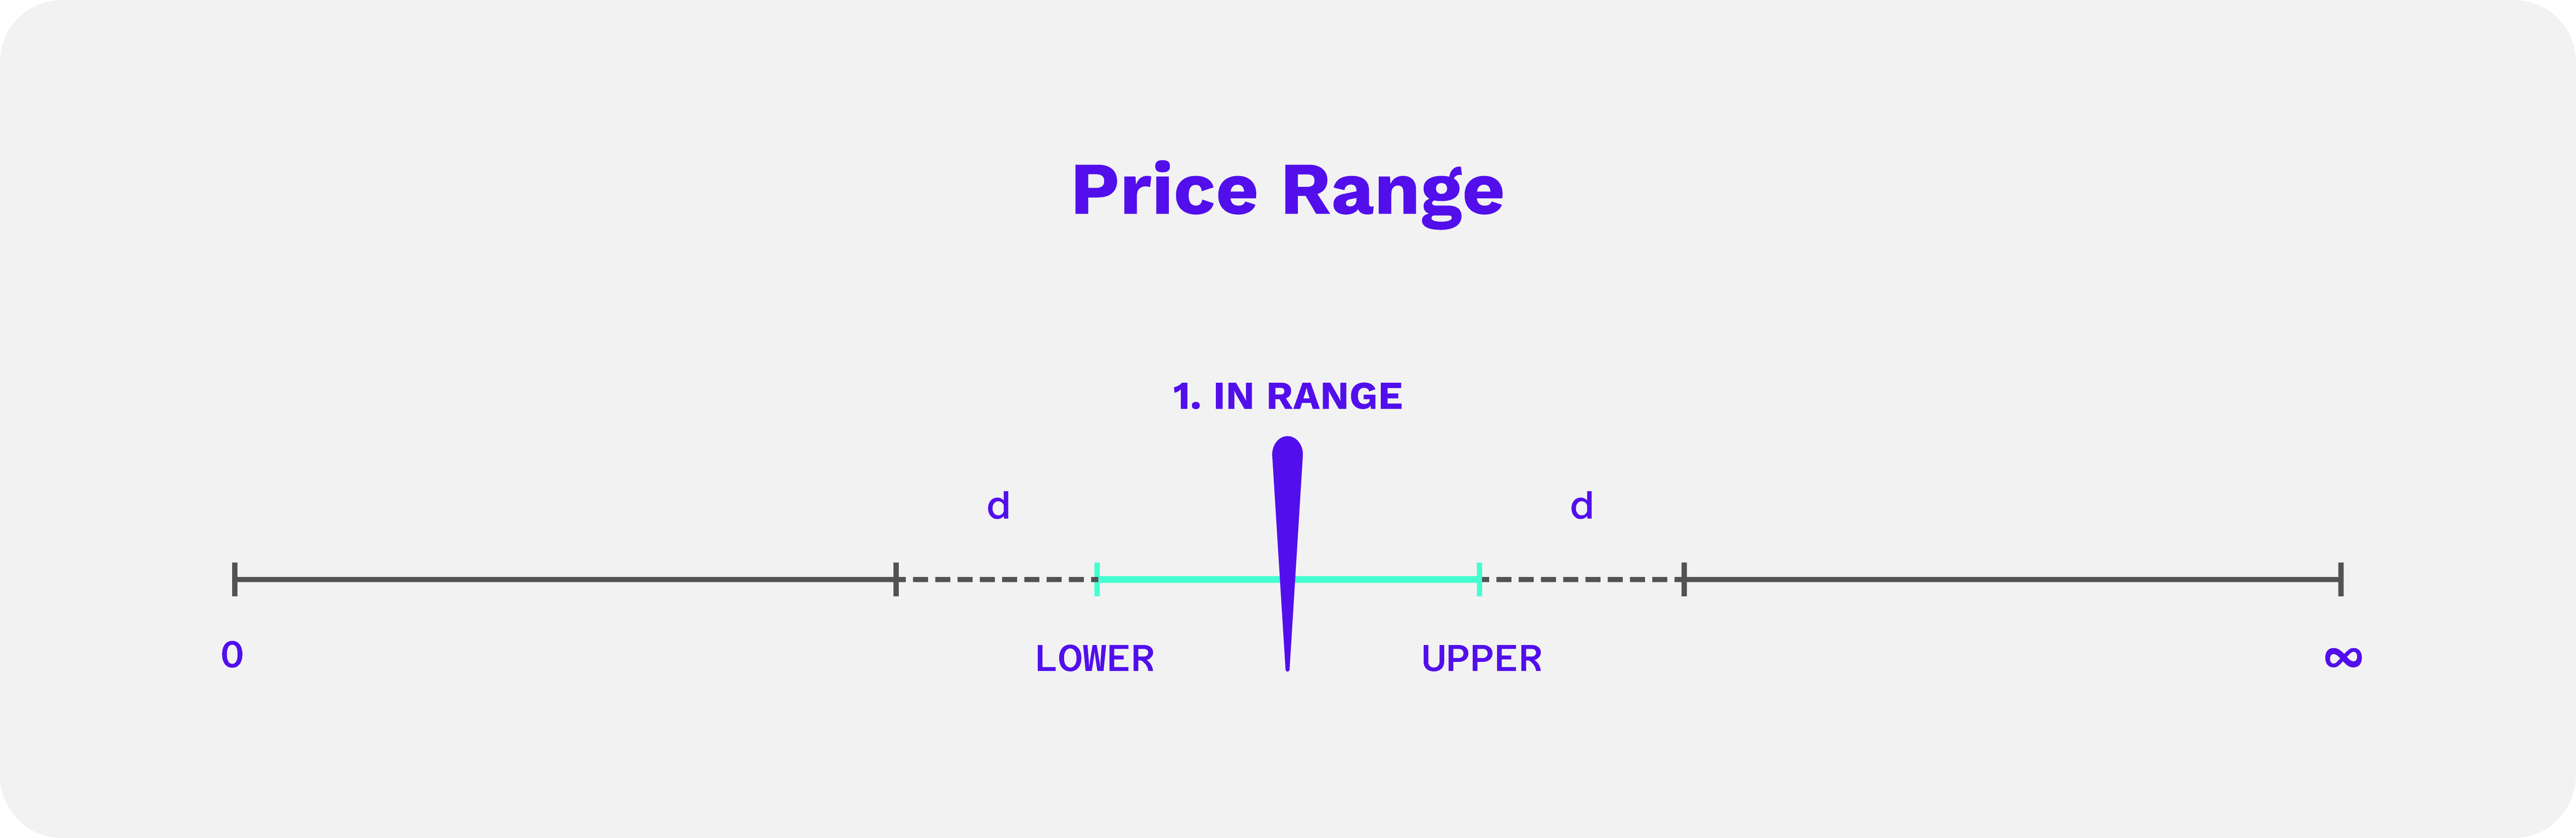
\includegraphics[scale=0.3]{in_range.png}
  \centering
  \caption{Esempio di posizione in range - Orbit Documentation}
  \label{fig:in_range}
\end{figure}

\noindent \\Possiamo invece trovarci nella situazione della figura \ref{fig:oor}, dove il prezzo attuale del rapporto della coppia dei Token della pool si trova al di fuori del range scelto inizialmente dall'utente.\\

\begin{figure}[H]
  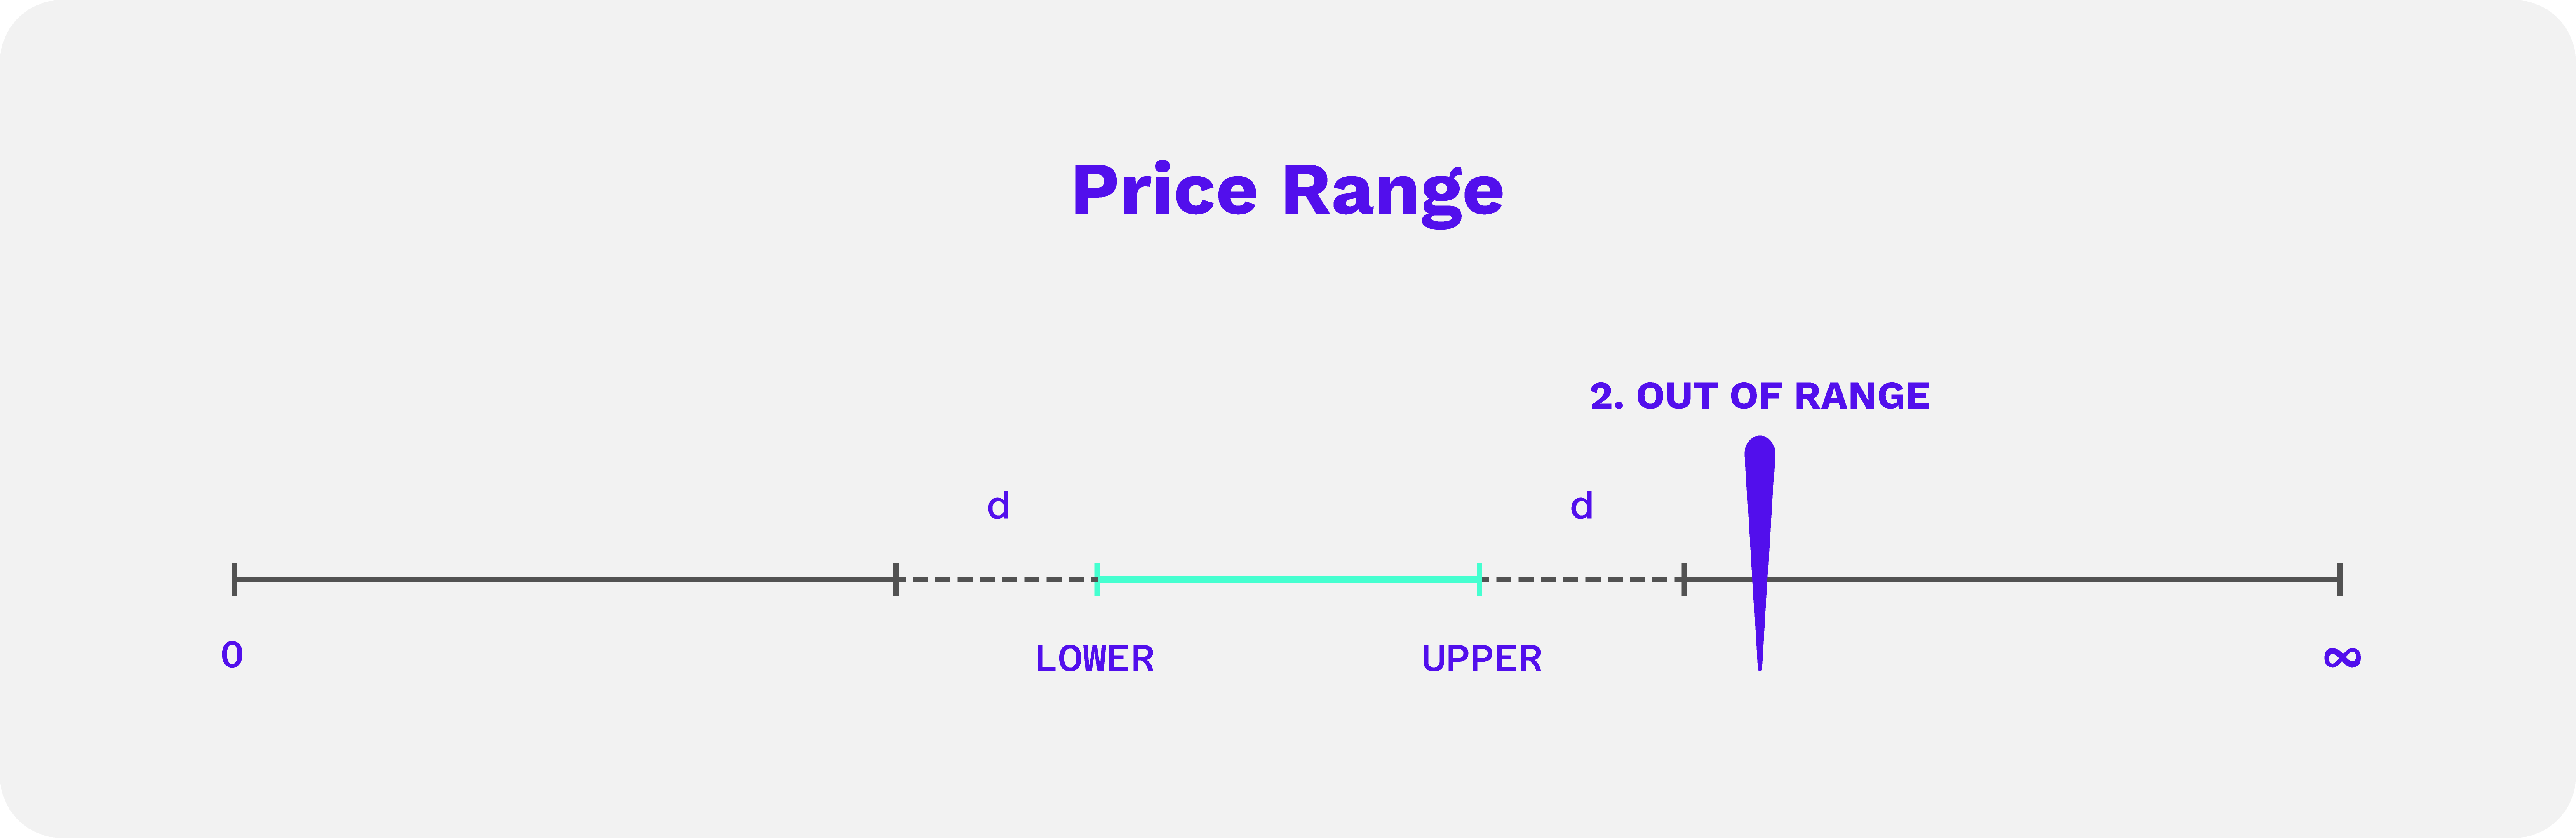
\includegraphics[scale=0.3]{oor.png}
  \centering
  \caption{Esempio di posizione fuori range - Orbit Documentation}
  \label{fig:oor}
\end{figure}

\noindent \\In questo caso, una volta superata la soglia delimitata dai due segmenti $d$, estensioni del \textbf{lower e upper bound} dell'intervallo di prezzo, il modulo di autorebalance viene innescato, impostando un nuovo range di prezzo \textbf{centrato sul prezzo attuale} (figura \ref{fig:new_range}).
In questo modo gli utenti non smettono mai di guadagnare fee, nonostante il prezzo possa variare molto rispetto al range scelto alla creazione della posizione.

\begin{figure}[H]
  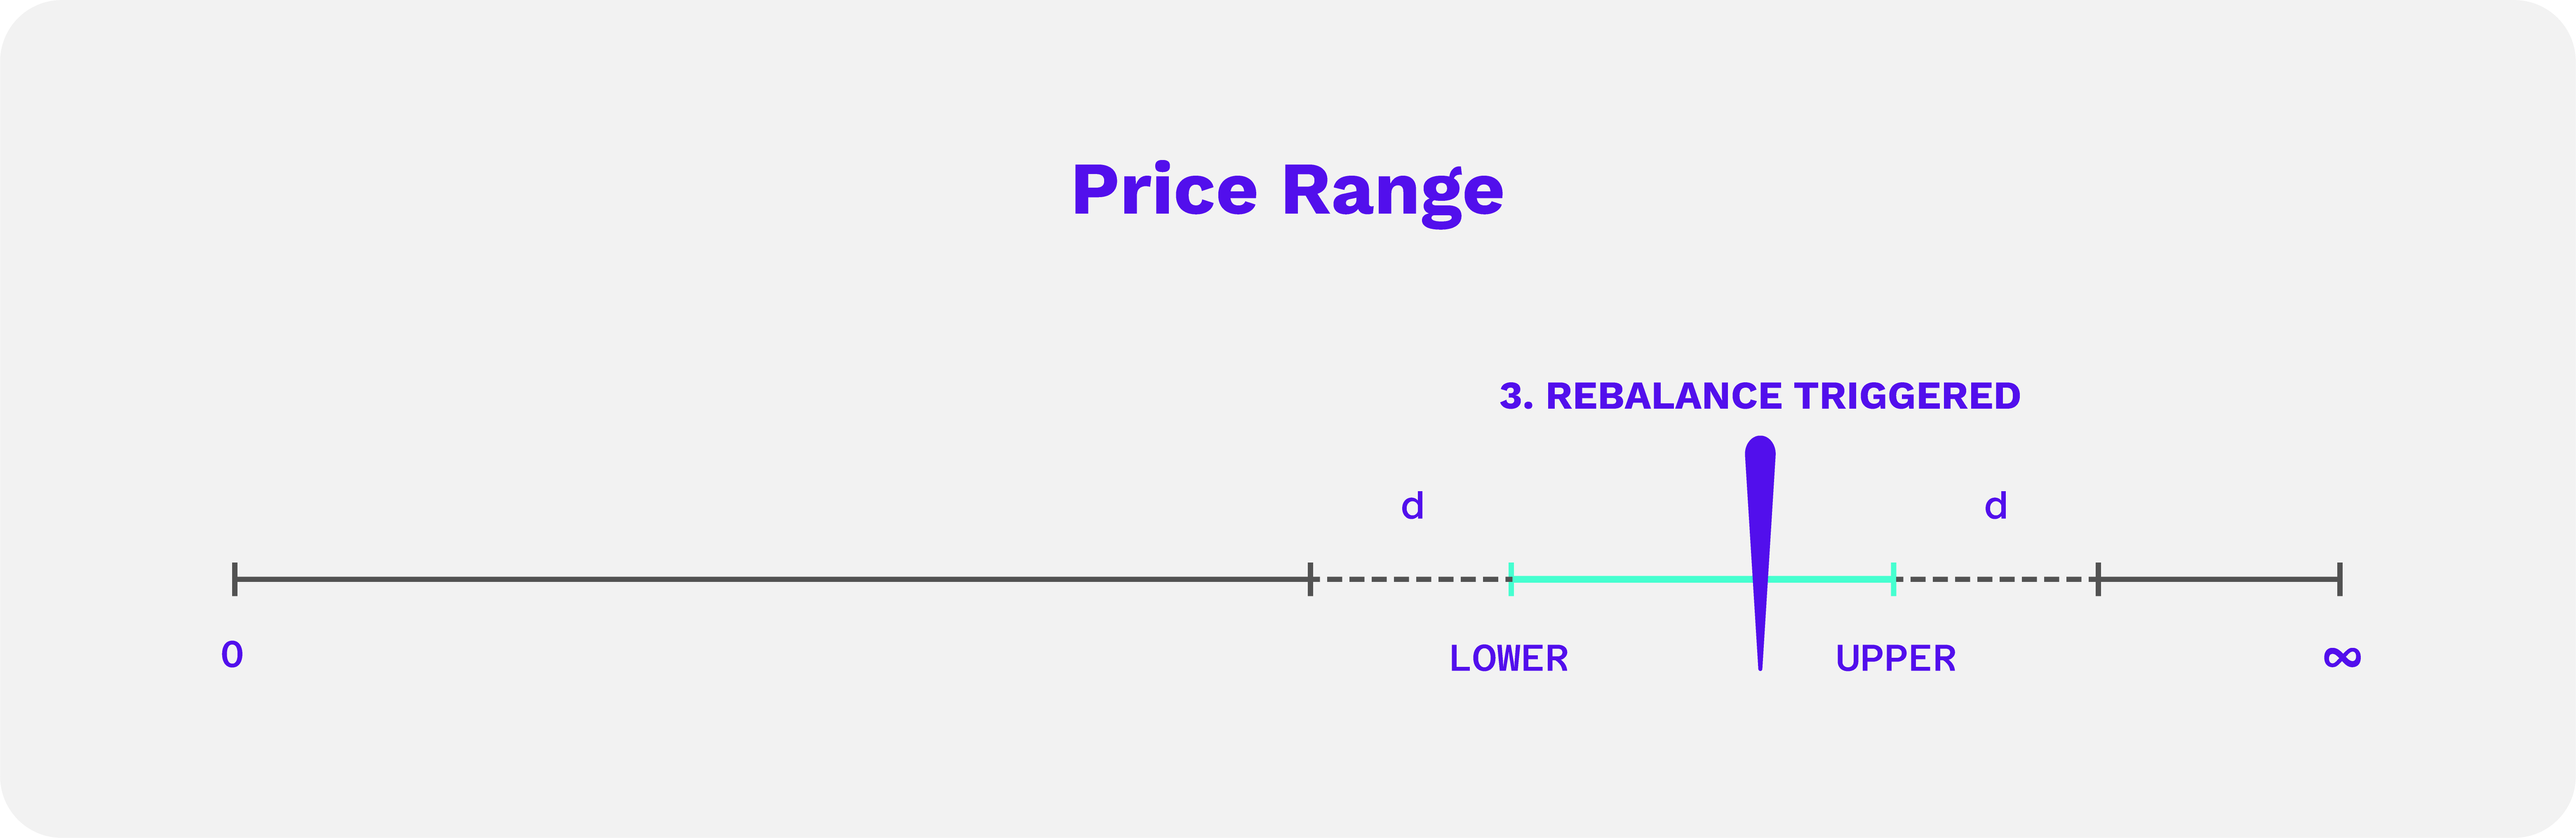
\includegraphics[scale=0.3]{new_range.png}
  \centering
  \caption{Nuovo range dopo l'attivazione del modulo di autorebalance - Orbit Documentation}
  \label{fig:new_range}
\end{figure}

\subsection{Idle liquidity module}

L'ultimo modulo di Orbit, \textbf{Idle liquidity module}, affronta sempre il problema della liquidità inattiva, ma adottando una diversa strategia rispetto all'autorebalance.
\\Il suo innesco avviene comunque quando il prezzo attuale del rapporto dei due token in una pool si trova al di fuori del range scelto per una determinata posizione. \\Quando ciò accade, la liquidità della posizione viene trasferita su altri protocolli (al di fuori di Uniswap V3), come per esempio \textbf{Aave Protocol}, attualmente implementato su Orbit (figura \ref{fig:aave}).

\begin{figure}[H]
  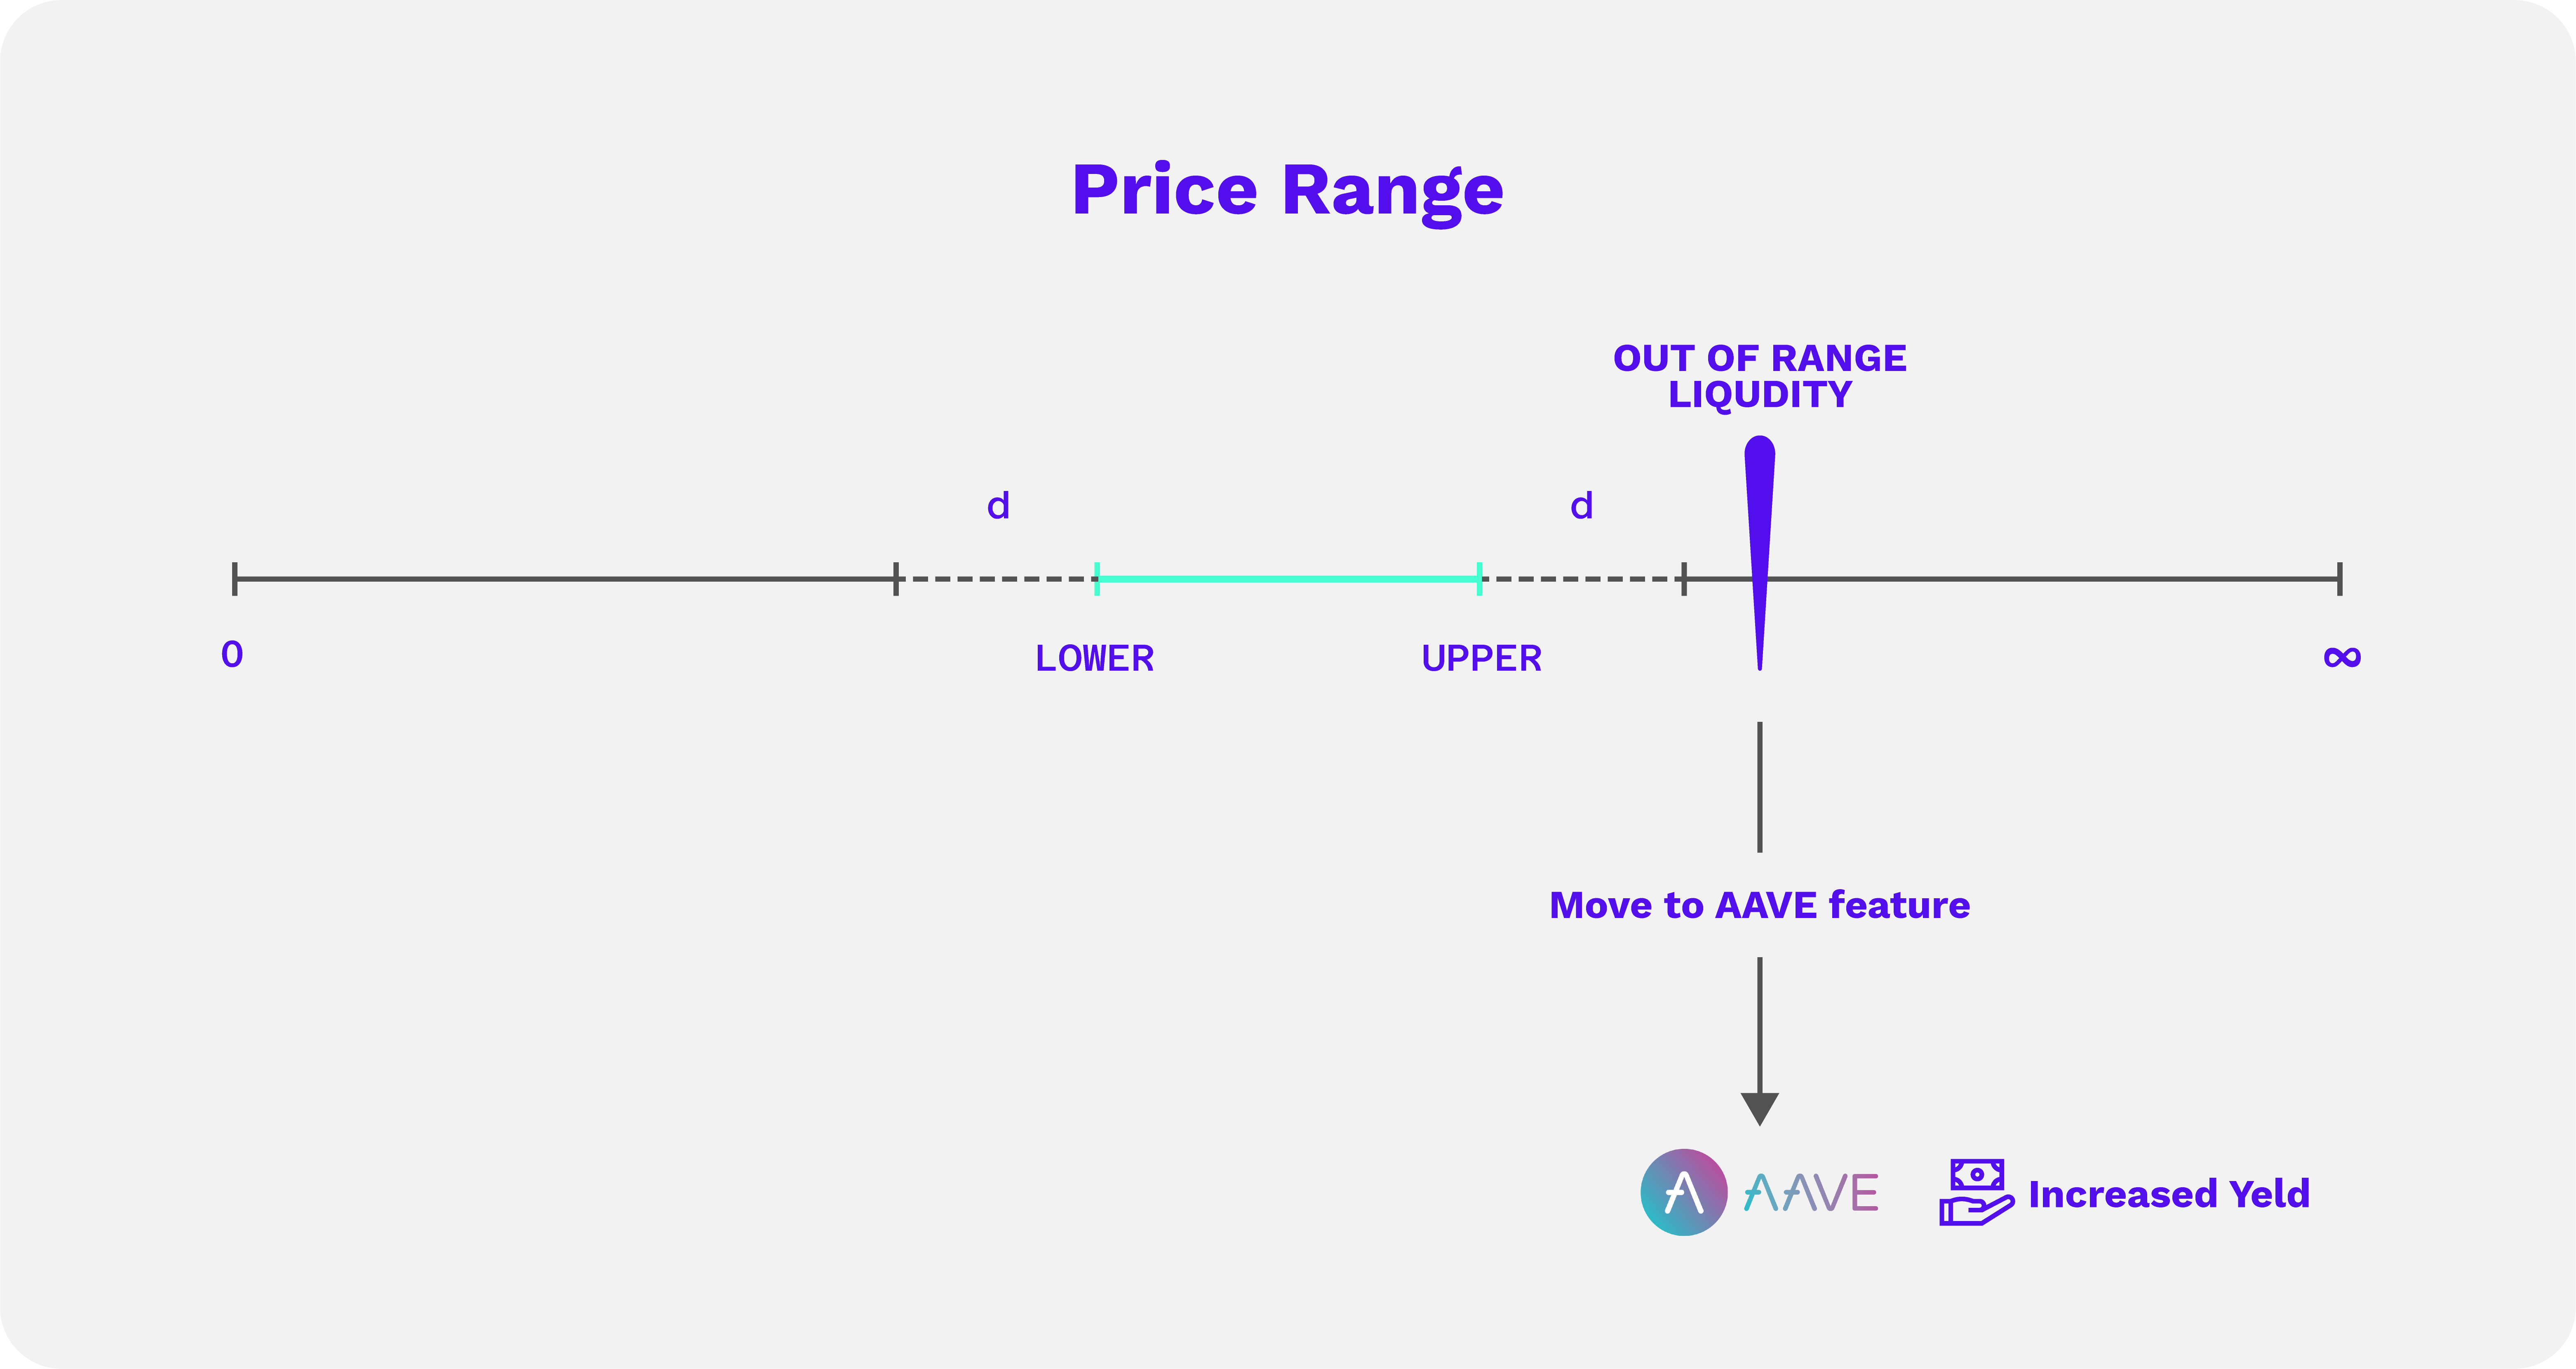
\includegraphics[scale=0.3]{aave.png}
  \centering
  \caption{Liquidità inattiva spostata su Aave - Orbit Documentation}
  \label{fig:aave}
\end{figure}


\noindent \\Tali protocolli permettono all'utente di usufruire di modi alternativi di guadagnare fee sulla liquidità fornita, così da rendere proficua la posizione nonostante si trovi al di fuori dell'intervallo prestabilito.
Una volta che il prezzo torna nell'intervallo scelto dall'utente, la posizione sugli altri protocolli viene chiusa, e nuovamente aperta su Uniswap V3, come mostrato in figura \ref{fig:uniswap_back}.

\begin{figure}[H]
  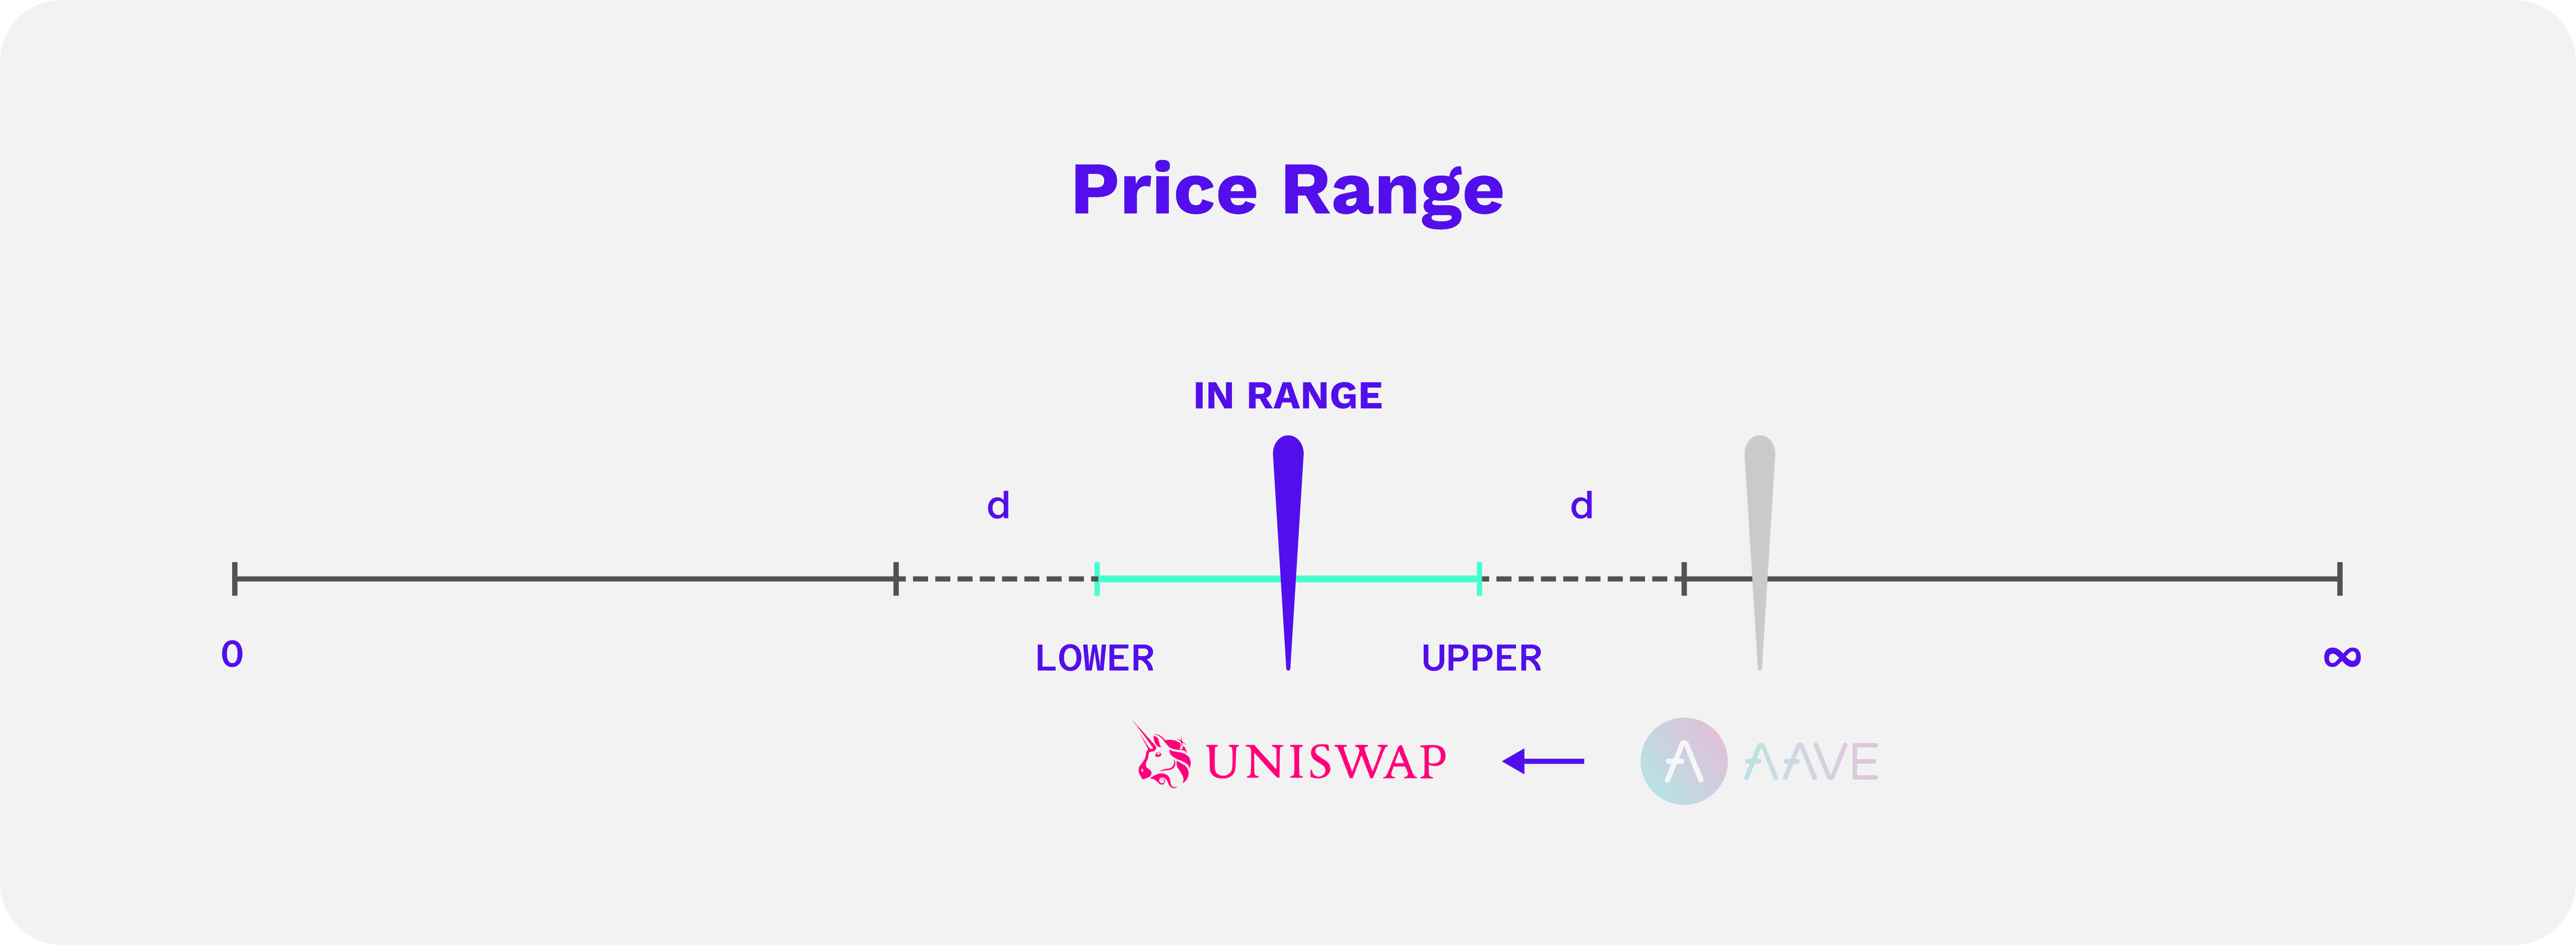
\includegraphics[scale=0.3]{uniswap_back.png}
  \centering
  \caption{Posizione chiusa su Aave ma riaperta su Uniswap V3 - Orbit Documentation}
  \label{fig:uniswap_back}
\end{figure}

\noindent \\Per ovvie ragioni logistiche, il modulo di autorebalance e quello di idle liquidity sono \textit{mutualmente esclusivi}, dunque non possono essere contemporaneamente attivi su una stessa posizione.
\chapter{Tecnologie utilizzate nello sviluppo di Orbit}

Orbit è una piattaforma che prende forma nel mondo del Web3, pertanto per la sua realizzazione sono state richieste tecnologie specifiche di questo emergente settore.
\\Possiamo logicamente suddividere Orbit in due macro parti: il \textbf{frontend}, ossia l'interfaccia della dApp\cite{orbit_website} con la quale l'utente interagisce direttamente, ed il \textbf{backend} composto da una suite di contratti che racchiudono le logiche e meccanismi su cui Orbit si basa.

\section{Tecnologie Frontend e librerie utilizzate}

La scelta del linguaggio utilizzato per la dApp Orbit, trattandosi di un'applicazione web, è ricaduta sul linguaggio \textbf{Javascript}\cite{js}.\\Le caratteristiche del linguaggio, quali \textit{versatilità, leggerezza e facilità d'apprendimento} hanno condizionato questa scelta.
\\\\Inoltre, a seguito di uno studio di mercato riguardante le librerie utilizzate dalle moderne dApps, incrociato con le competenze degli sviluppatori del team di Five Elements Labs, sono state selezionate una serie di librerie coerenti con lo il linguaggio scelto.
\\\\Lo sviluppo del frontend di Orbit e la relativa interazione con wallet e smart contracts è stato il principale compito affidatomi durante il mio Project Work.

\subsection{Elementi dell'interfaccia}

Per la creazione degli elementi che formano l'interfaccia di Orbit, è stata scelto \textbf{ReactJS}\cite{react}, una libreria Javascript per la sviluppo di \textbf{Single Page Application} (SPA\cite{spa}), che permette la creazione di componenti flessibili e riutilizzabili, nonché la più utilizzata nel 2021 tra le librerie web secondo \textit{StackOverflow}\cite{react_2021} (figura \ref{fig:react}).

\begin{figure}[H]
  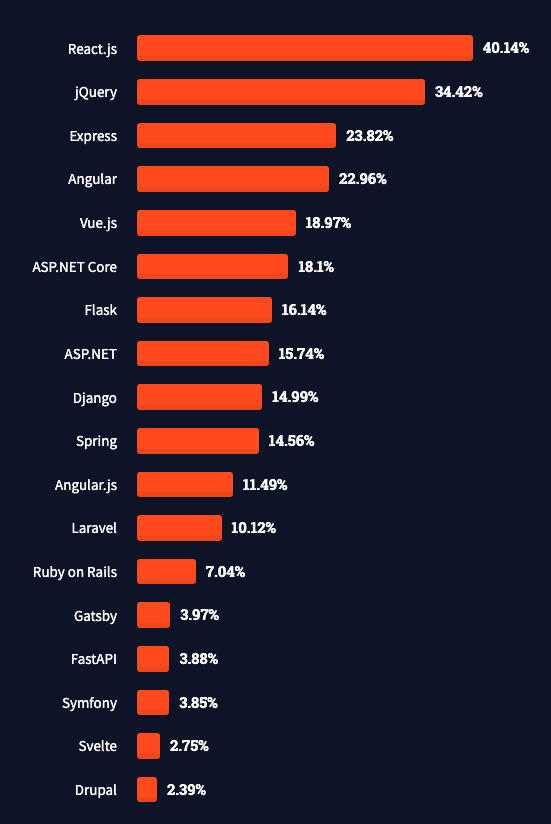
\includegraphics[scale=0.45]{react.png}
  \centering
  \caption{Librerie web più utilizzate del 2021 secondo un report di Stack Overflow}
  \label{fig:react}
\end{figure}


\noindent\\Per quanto riguarda invece lo stile dei componenti è stata utilizzata \textbf{Tailwind CSS}\cite{tailwind} un framework CSS che permette di utilizzare classi per il layout, colori, tipografia e altre caratteristiche stilistiche dell'interfaccia grafica.

\subsection{Interazione con gli Smart Contracts}

Ciò che più differenzia un'applicazione web2 da una dApp in Web3 è l'interazione con gli Smart Contracts.\\La libreria scelta per tale interazione è stata \textbf{ethers.js}\cite{ethers}: come suggerisce il nome, si tratta di una libreria Javascript che mira a facilitare l'interazione con la Blockchain di Ethereum (nel nostro caso, Polygon).
\\Tra le sue molteplici funzionalità, vi sono la \textit{connessione di un wallet} alla dApp, la \textit{creazione di istanze di oggetti che rappresentano Smart Contracts} utilizzabili direttamente nel Frontend ed infine la \textit{firma dei messaggi relativi alle transazioni}.

\section{Connessione wallet to wallet}

Analogamente all'interazione \textit{"Client-Server"} del web tradizionale, vi è un'interazione \textit{Wallet-to-Wallet} nel Web3. Ogni utente più avere uno o più wallet digitali, ciascuno dei quali viene identificato da un indirizzo (\textbf{Ethereum Address}) a \textbf{42 caratteri alfanumerici}. Tra questi, 40 sono in formato numerico esadecimale e i restanti 2 compongono il prefisso \textbf{0x}.
\\\\A questo punto, è lecito chiedersi come possa un wallet interagire con gli Smart Contracts di Orbit.\\
Nello stesso modo in cui i wallet possono comunicare tra loro, ossia attraverso l'invio e ricezione di transazioni, anche uno Smart Contract può ricevere delle transazioni, essendo identificato sulla blockchain con un proprio indirizzo esadecimale.
\\\\Per fare un esempio, lo Smart Contract del token \textbf{WETH} presente sulla rete Polygon, si trova all'indirizzo:\\
\[ 0x7ceb23fd6bc0add59e62ac25578270cff1b9f619 \]
\\Ciò significa che se un wallet volesse interagire con il contratto, magari per controllare l'ammontare di WETH che possiede, dovrebbe inviare una transazione a tale indirizzo. Dunque, a seconda dei parametri impostati, verrà eseguirà una specifica funzione presente nello Smart Contract, che potrebbe utilizzare con i dati presenti in esso, modificandoli o inviandoli al mittente della transazione.

\subsection{Metamask e Wallet Connect}
\\\\Per dare la possibilità ad un utente di connettere il proprio wallet ad Orbit ed effettuare le operazioni appena discusse, è stato scelto di implementare due sistemi: il primo, forse più noto nel Web3, è il wallet per criptovalute \textbf{Metamask}\cite{metamask} mentre il secondo è il protocollo \textbf{WalletConnect}\cite{walletconnect}.
\\\\Metamask non è solo un wallet digitale, ma un vero e proprio \textit{gateway} per interagire con applicazioni decentralizzate. Come si può vedere nella figura \ref{fig:metamask}, si presenta come un'estensione del browser, dalla quale si può gestire più wallet personali presenti su blockchain diverse, visualizzare lo storico delle transazioni effettuate, l'ammontare dei token ERC-20 posseduti dall'utente ed effettuare transazioni.\\
\begin{figure}[H]
  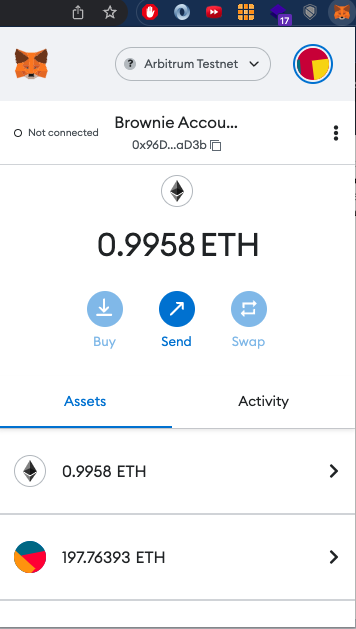
\includegraphics[scale=0.6]{metamask.png}
  \centering
  \caption{Screenshot di uno dei miei personali wallet su Metamask, estensione browser}
  \label{fig:metamask}
\end{figure}
\noindent \\WalletConnect è invece un protocollo che permette di integrare all'interno della propria dApp più tipologie di wallet (tra i quali anche Metamask).\\Le principali caratteristiche di WalletConnect sono \textbf{adattabilità} e \textbf{facilità di integrazione} con un qualsiasi portafoglio digitale: basterà che l'utente selezioni la propria wallet app o che inquadri un QR Code per effettuare immediatamente la connessione alla dApp di Orbit. 
\\\\Inoltre, è una valida soluzione per facilitare la connessione ad una dApp da dispositivi mobili, che allo stato attuale risulta ostica per la maggior parte dei prodotti Web3.

\subsection{Usabilità del sistema}

Nei mesi precedenti al lancio del prodotto, è stato svolto un importante lavoro di analisi di usabilità per rendere Orbit una piattaforma quanto più accessibile per i propri utenti, svolgendo delle sessione di \textbf{Beta Testing}, attraverso le quali sono sorti dubbi e feedback che hanno estremamente semplificato il flusso utente del prodotto finale. 
\\\\In quest'ultima parte, sono riuscito a dare il mio contributo attraverso nozioni imparate nel mio percorso di studi, in particolare in \textit{Interazione Uomo-Macchina}, quali principi di design dell'usabilità, scelta di palette cromatiche inclusive per persone con anomalie visive quali il daltonismo ed euristiche per facilitare l'esperienza utente.  

\section{Tecnologie Backend}

Il Backend è ciò che l'utente non vede concretamente, ma che contiene la logica applicativa di Orbit, costruita sopra una suite di Smart Contracts che ricoprono le principali funzionalità della piattaforma.

\subsection{Solidity}

Per lo sviluppo degli Smart Contracts di Orbit è stato scelto \textbf{Solidity}\cite{solidty}, il linguaggio di programmazione che viene utilizzato per sviluppare la maggior parte delle tecnologie blockchain presenti sul mercato. Nonostante la sua iniziale difficoltà di apprendimento, l'ecosistema di Solidity permette di avere una vasta scelta di librerie e contratti consolidati su cui basare i propri progetti.
\\Si tratta di un linguaggio \textit{orientato agli oggetti}, di alto livello e che supporta \textit{complessi tipi di oggetti} definiti dallo sviluppatore, ideale per ospitare ogni tipo di strutture dati.
\\\\Tuttavia, come già accennato nel capitolo precedente, le blockchain \textbf{Ethereum-based} hanno un costo computazionale rilevante, misurato in gas. Per questa ragione bisogna prestare particolare attenzione quando si utilizzano linguaggi come Solidity, in quanto una semplice \textbf{implementazione di una funzione} mal realizzata potrebbe richiedere un costo extra che, a seconda della rete in cui ci si trova, potrebbe risultare in un'importante spesa per il il mittente della transazione.

\subsection{Hardhat}

Data la delicatezza e fragilità dello sviluppo di una suite di Smart Contracts, è necessario avere uno strumento per testarne le principali funzioni, possibilmente prima che essi vengano rilasciati sulla blockchain. Proprio per questo è stato scelto di utilizzare \textbf{Hardhat}\cite{hardhat}, un ambiente di sviluppo per costruire software sulla blockchain di Ethereum, il quale comprende diverse librerie che sinergizzano alla perfezione con lo sviluppo di Smart Contracts.\\\\\textbf{Hardhat Runner} è una tra queste: viene utilizzato per costruire dei \textbf{task}, ossia azioni eseguibili tramite linea di comando.
Per esempio, sono state realizzate specifiche azioni per compilare il codice degli Smart Contracts, eseguire dei test su di essi e distribuirli (\textit{deploy}) sulla rete locale di Hardhat.
\\Infatti, uno dei tanti vantaggi di Hardhat è quello di testare i propri contratti su una rete locale, contenente 20 indirizzi utilizzabili per effettuare transazioni verso i propri Smart Contracts, al fine di avere un ambiente che preceda quello di produzione.
\\Inoltre, sono stati realizzati decine di test per ogni funzione dei contratti di Orbit, realizzati nel linguaggio \textbf{Typescript} che, a differenza di Javascript, ha un forte controllo sulla tipizzazione delle variabili, costruzione di interfacce e fornisce una sicurezza maggiore nello sviluppo.
\\\\Per la costruzione delle Test Suite sono state utili delle nozioni imparate durante il corso di \textit{Sicurezza e Affidabilità}, che mi ha permesso di dare un contribuito nel lavoro svolto dai miei colleghi nello sviluppo dei contratti.


\chapter{Architettura di Orbit}

Durante i mesi di sviluppo di Orbit, sono state effettuate numerose ricerche da parte della squadra di sviluppo di Five Elements Labs, in modo tale da scegliere un'architettura e dei \textbf{design patterns} quanto più sicuri e aggiornati con le ultime tecnologie del mondo DeFi e Smart Contracts.

\section{Principi fondamentali}

L'architettura su cui si basa Orbit segue due principi fondamentali: \textbf{composability} (componibilità) e \textbf{upgradability} (aggiornabilità).
\\\\Il primo principio afferma che i componenti che formano un sistema software debbano essere realizzati in modo tale da poter essere riutilizzabili, per costruire nuove applicazioni. Un buon esempio di questo principio è quello dei mattoncini \textit{Lego}: gli Smart Contracts di Orbit sono dei singoli mattoncini che combinati tra loro possono costruire strutture sempre più complesse, senza la necessità di essere riscritti da zero.
\\\\Il secondo principio invece, riguarda l'aggiornabilità di alcune funzionalità degli Smart Contracts. Gli Smart Contracts su \textbf{EVM}\cite{evm} eseguono solo il codice per cui sono programmati al momento del loro \textit{deploy} sulla blockchain. \\Tuttavia, attraverso il Design Pattern adottato da Orbit, è possibile aggiornare alcune loro funzionalità tramite contratti esterni, abbattendo i costi di distribuzione sulla blockchain (approfondimento nella sezione \ref{registry}).

\section{Diamond Pattern}

L'architettura presenta numerosi Smart Contracts, ognuno di essi adibito ad una specifica funzione all'interno della suite.
\\Il design pattern utilizzato è chiamato \textbf{Diamond Pattern}\cite{diamond} (figura \ref{fig:contracts_flow}) o standard EIP-2535. Si tratta di un approccio che consiste nella costruzione di un sistema di Smart Contract \textbf{modulari}, \textbf{estendibili} ed \textbf{aggiornabili}, contenuti in  un spazio di memoria \textit{virtualmente infinito}.



\begin{figure}[H]
  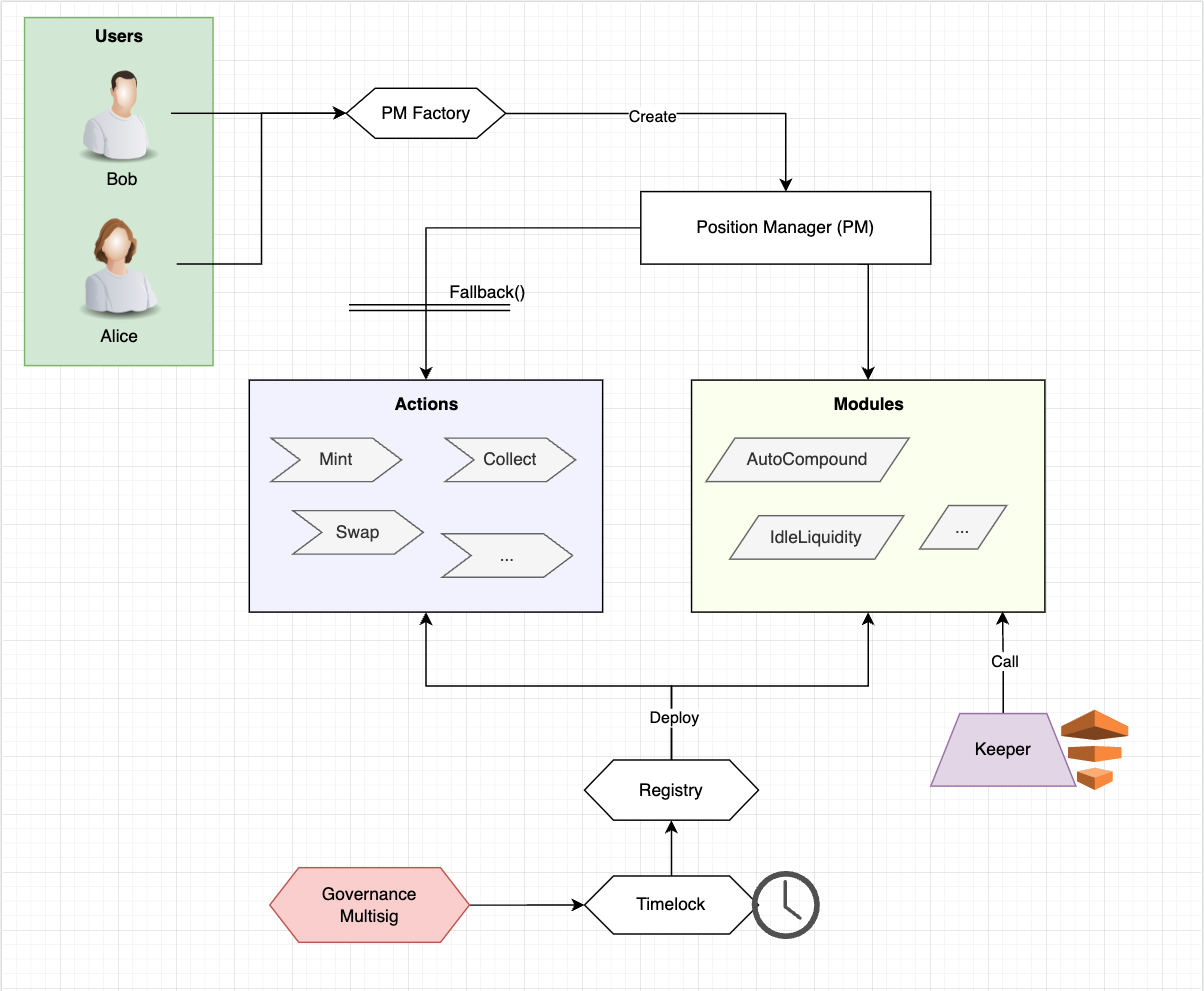
\includegraphics[scale=0.40]{contracts_flow.png}
  \centering
  \caption{Architettura degli Smart Contracts di Orbit}
  \label{fig:contracts_flow}
\end{figure}


\subsection{Vantaggi del Diamond}

Il Diamond Pattern è uno standard recente, che ha trovato largo uso nel mondo Web3.
\\Il vantaggio principale sta nello sfruttare un \textbf{singolo smart contract} (chiamato Diamond), dunque un solo indirizzo ethereum, per contenere tutte le funzionalità alle quali possono accedere i contratti presenti nell'architettura.
\\Seppur tale contratto sia soggetto alla canonica limitazione di dimensione di \textbf{24KB}, può fare affidamento a codice presente su contratti esterni, rendendo lo spazio a sua disposizione \textbf{virtualmente infinito}. 
\\\\Non meno importante è la sua \textbf{mutabilità}: tutte le funzioni di tipo "\textit{external}", ossia chiamabili da altri contratti, possono essere modificate, eliminate o aggiunte in un qualsiasi momento senza dover distribuire nuovamente il contratto sulla blockchain, evitando costi aggiuntivi e l'utilizzo di un nuovo indirizzo.

\subsection{Creazione, aggiornamento e eliminazione di funzioni}

Il \textbf{Diamond Pattern} possiede una forte \textbf{modularità}. \\Vi sono funzioni "\textit{external}", messe a disposizione da ulteriori contratti stateless chiamati \textbf{Facet}.
\\In questo caso, vi è un chiaro parallelismo tra il mondo reale e le nomenclature utilizzate nell'architettura: nel settore industriale i diamanti vengono tagliati creando delle sfaccettature (Facets), proprio come nel Diamond Pattern sono "tagliati" aggiungendo, modificando e eliminando funzioni dai Facets. \\I contratti Facet vanno visti come entità separate, indipendenti tra loro ma che condividono l'accesso alle stesse funzioni, librerie e variabili di stato.
\\Quando un Facet viene distribuito sulla blockchain, deve essere aggiunto al Diamond tramite una transazione che ne specifica i dettagli (ad esempio, le firme di una collezione di funzioni chiamabili su quel Facet). In questo modo, il Diamond potrà eseguire il codice presente nelle funzioni del Facet, utilizzando il suo stesso storage.



\subsection{Funzioni di fallback}

Quando viene chiamata una funzione dal Diamond, è di conseguenza innescata una particolare funzione detta di \textbf{fallback}. Tale funzione determina quale Facet verrà chiamato, in base ai primi \textit{4 bytes di dati}, detti \textit{function selector} (figura \ref{fig:facet}), per poi eseguire la funzione richiesta tramite il metodo \textbf{delegatecall}.
\\La funzione di fallback e il metodo delegatecall permettono ad un Diamond di eseguire una funzione di un Facet come se fosse implementata nel Diamond stesso. 
\\Inoltre è possibile chiamare differenti Facet in una singola transazione, risparmiando notevoli quantità di Gas, raggruppando dati e funzionalità nel singolo Diamond.

\begin{figure}[H]
  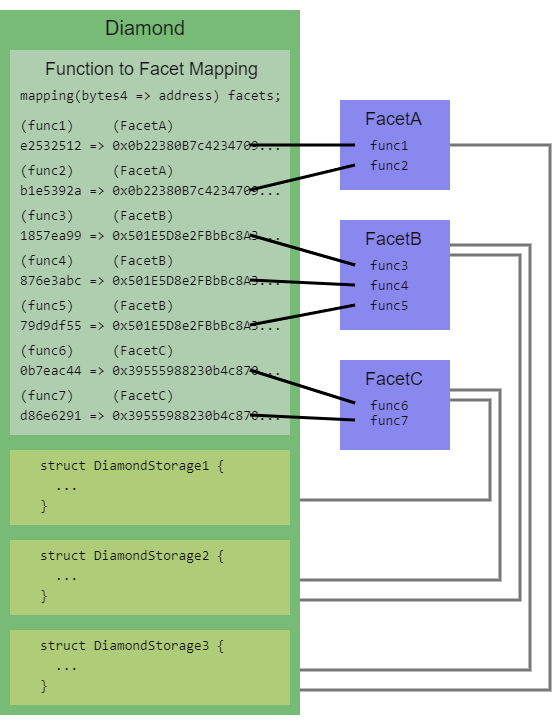
\includegraphics[scale=0.35]{facet.png}
  \centering
  \caption{Mapping tra function selector e funzioni dei contratti Facet - EIP-2535\cite{diamond}}
  \label{fig:facet}
\end{figure}


\subsection{Storage}

\todo{il discorso storage va sistemato meglio, non è una limitazione di solidity ma un problema di collisione}
Il sistema che gestisce lo spazio di archiviazione (da ora in poi \textbf{storage}) di Solidity non supporta contratti proxy come il Diamond. Per tale ragione, è necessario implementare uno speciale storage associato al Diamond, appositamente creato per interagire con i Facet. 
\\Quest'ultimi possono condividere l'accesso alle variabili di stato dello storage, usando le stesse strutture dati, che si devono trovare nelle stesse posizioni delle celle di memoria per essere accedute. In questo modo i Facet agiscono come entità separate ma con una memoria condivisa.





\subsection{Position Manager}

Il contratto che rappresenta lo Smart Vault creato dall'utente è chiamato \textbf{Position Manager}. Il suo compito principale è di gestire le posizione di Uniswap V3 appartenenti all'utente, salvando all'interno di una struttura dati quali moduli (\textit{autocompound, autorebalance, idle liquidity}) sono stati attivati per una relativa posizione.
L'unico punto di ingresso lato utente è rappresentato dall'interazione diretta con un contratto chiamato "\textit{PositionManagerFactory}", il quale si occupa della creazione dei Position Manager (interazione mostrata nella figura \ref{fig:contracts_flow}).


\subsection{Action}

Gli \textbf{Action} sono Smart Contract che contengono una singola funzione basilare; sono visti come dei singoli "\textit{mattoncini}" che costituiscono le strategie proposte all'utente.
\\Sono estensioni del contratto \textbf{BaseAction} il quale presenta un'unica funzione \textbf{doAction} che accetta un array di byte in input e restituisce un secondo array di byte in output.
\\

Actions are smart contracts which contain a single base function of our product. They are thought to be the building blocks of user's strategy and to be easily interactable with other contracts.

Problem
There are some basic functions we want to be accessible from multiple contracts, and this is a way to avoid duplicate code while also improving the composabiliy. The idea is to build simple blocks of basic operations which can be rearranged as the product evolves.

The Pattern
Actions are build on the same contract BaseAction to have uniform input and output types (bytes[]) and main functions. Actions extend this contract introducing the functionality and the functions to manage input/output conversion.

Since they will be composed by other modules to perform user's strategy they should be pretty basic, but not all functions should be actions: allowing the user to customize their strategy too much would result in a poor user expericence. For example, we want a user to be able to mint a UniV3 position, or perform a swap, but we don't want to give them the option to approve (or not to approve) tokens before each of those actions (since we would like to automate that process).

SPIEGO QUALI SONO E COME VENGONO GESTITE LE ACTIONS

\subsection{Moduli}

SPIEGO COME VENGONO GESTITI I MODULI

\subsection{Helpers}

Gli \textbf{Helpers} sono particolari librerie o funzioni utilizzabili più volte nel codice.
L'implementazione di tali librerie rispetta il principio \textbf{DRY} (don't repeat yourself), evitando di scrivere codice duplicato all'interno degli Smart Contracts.
\\Invece, è possibile utilizzare le funzioni degli Helpers importando solo ciò di cui abbiamo bisogno negli opportuni contratti, senza dover riscrivere codice già esistente nella codebase.

\section{Sicurezza}

\subsection{Registry patterns} \label{registry}

\subsection{Timelock}

\section{Audit}

La dApp di Orbit è stata costruita dando priorità elevata alla sicurezza dei propri utenti. Per questa ragione è stata svolto un processo di \textbf{Audit}\cite{audit} da parte di \textit{ByteRocket}.
\\Un Audit è un'esaminazione metodica che comprende l'analisi del codice degli Smart Contracts di un prodotto. \\Tale processo ha come obiettivo la scoperta di errori, problematiche, falle alla sicurezza e potenziali vulnerabilità nel codice. A fine analisi, viene rilasciato un report in cui vengono suggeriti miglioramenti e modi per risolvere le vulnerabilità e bug, suddivisi per severità, come mostrato in figura \ref{fig:audit}. 

\begin{figure}[H]
  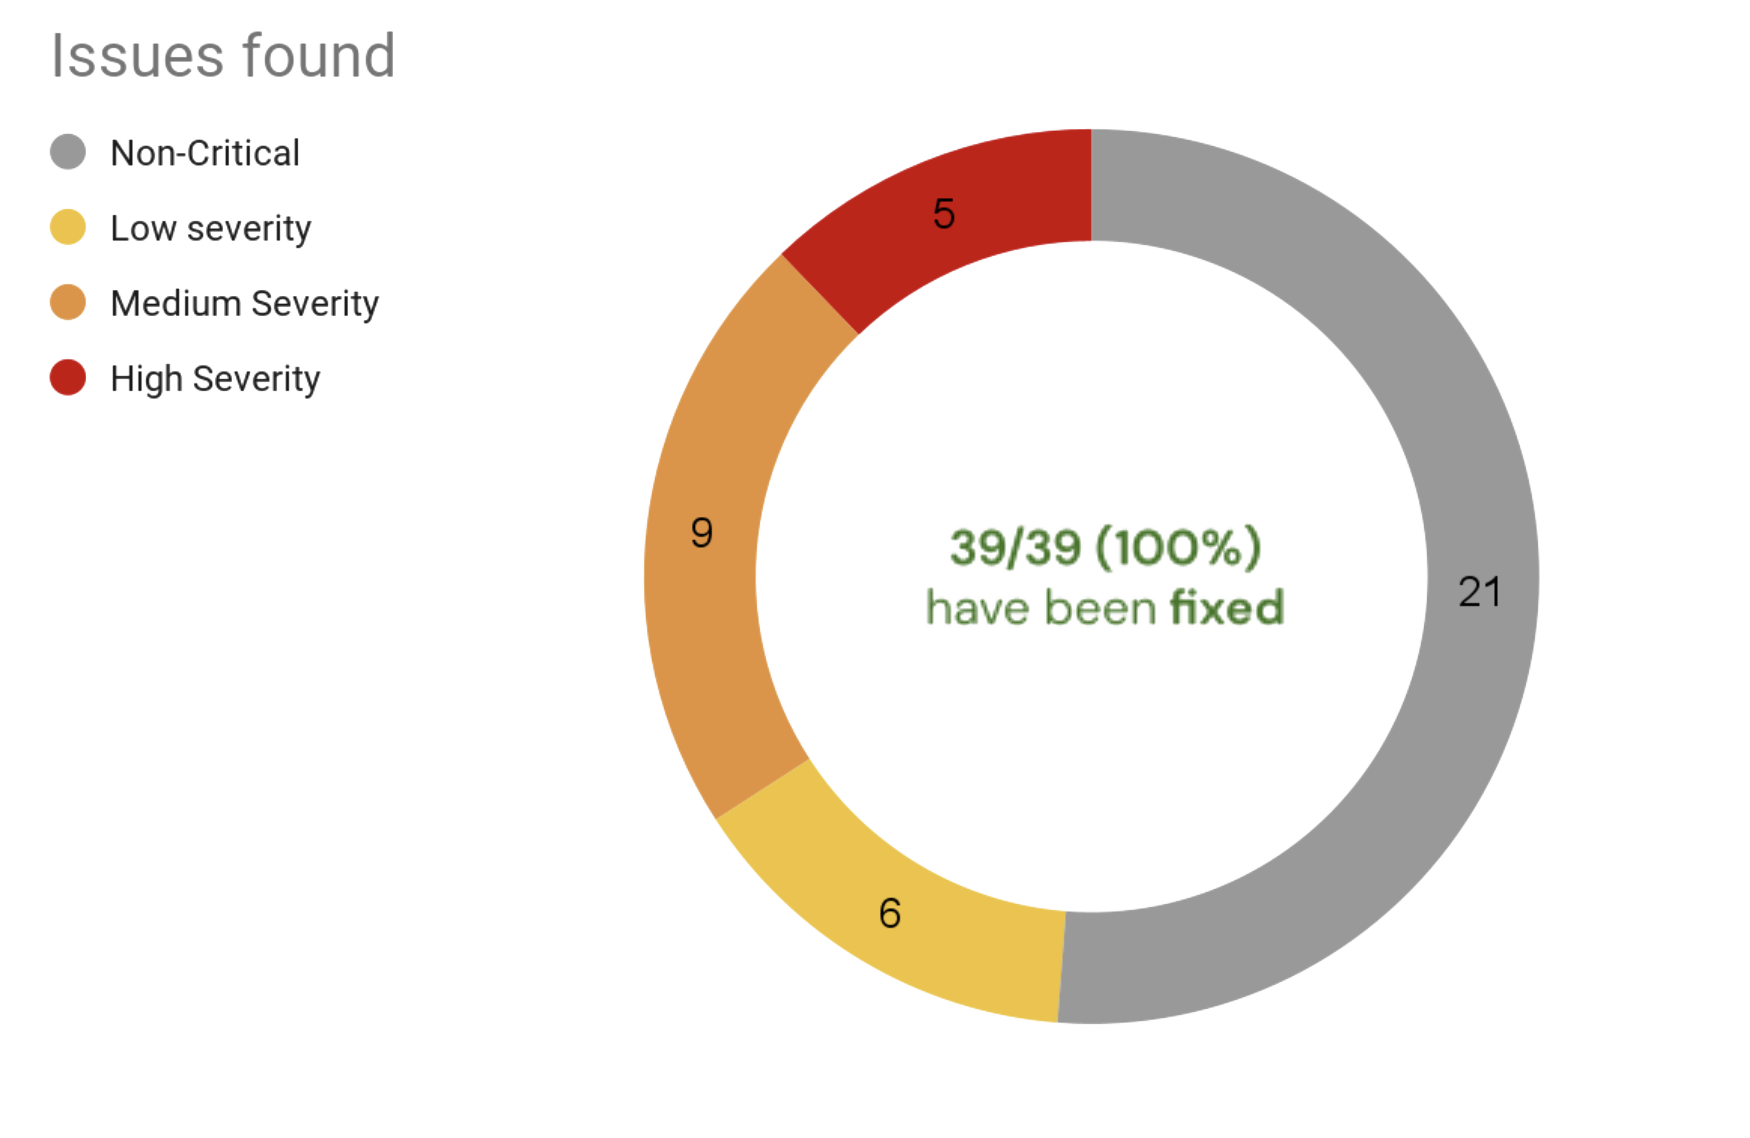
\includegraphics[scale=0.40]{audit.png}
  \centering
  \caption{Problemi rilevati da ByteRocket nella prima Audit di Orbit}
  \label{fig:audit}
\end{figure}

\noindent \\Come team di sviluppo, abbiamo risolto i 39 problemi trovati da ByteRocket, ottenendo una certificazione di completamento dell'Audit, al fine di garantire agli utenti di Orbit un elevato grado di sicurezza ed affidabilità.


\chapter{Future implementazione all'interno di Orbit}


\bibliographystyle{unsrtnat}
\bibliography{bibliografia}




\end{document}